% Options for packages loaded elsewhere
\PassOptionsToPackage{unicode}{hyperref}
\PassOptionsToPackage{hyphens}{url}
\PassOptionsToPackage{dvipsnames,svgnames,x11names}{xcolor}
%
\documentclass[
]{scrartcl}

\usepackage{amsmath,amssymb}
\usepackage{iftex}
\ifPDFTeX
  \usepackage[T1]{fontenc}
  \usepackage[utf8]{inputenc}
  \usepackage{textcomp} % provide euro and other symbols
\else % if luatex or xetex
  \usepackage{unicode-math}
  \defaultfontfeatures{Scale=MatchLowercase}
  \defaultfontfeatures[\rmfamily]{Ligatures=TeX,Scale=1}
\fi
\usepackage{lmodern}
\ifPDFTeX\else  
    % xetex/luatex font selection
\fi
% Use upquote if available, for straight quotes in verbatim environments
\IfFileExists{upquote.sty}{\usepackage{upquote}}{}
\IfFileExists{microtype.sty}{% use microtype if available
  \usepackage[]{microtype}
  \UseMicrotypeSet[protrusion]{basicmath} % disable protrusion for tt fonts
}{}
\makeatletter
\@ifundefined{KOMAClassName}{% if non-KOMA class
  \IfFileExists{parskip.sty}{%
    \usepackage{parskip}
  }{% else
    \setlength{\parindent}{0pt}
    \setlength{\parskip}{6pt plus 2pt minus 1pt}}
}{% if KOMA class
  \KOMAoptions{parskip=half}}
\makeatother
\usepackage{xcolor}
\setlength{\emergencystretch}{3em} % prevent overfull lines
\setcounter{secnumdepth}{5}
% Make \paragraph and \subparagraph free-standing
\makeatletter
\ifx\paragraph\undefined\else
  \let\oldparagraph\paragraph
  \renewcommand{\paragraph}{
    \@ifstar
      \xxxParagraphStar
      \xxxParagraphNoStar
  }
  \newcommand{\xxxParagraphStar}[1]{\oldparagraph*{#1}\mbox{}}
  \newcommand{\xxxParagraphNoStar}[1]{\oldparagraph{#1}\mbox{}}
\fi
\ifx\subparagraph\undefined\else
  \let\oldsubparagraph\subparagraph
  \renewcommand{\subparagraph}{
    \@ifstar
      \xxxSubParagraphStar
      \xxxSubParagraphNoStar
  }
  \newcommand{\xxxSubParagraphStar}[1]{\oldsubparagraph*{#1}\mbox{}}
  \newcommand{\xxxSubParagraphNoStar}[1]{\oldsubparagraph{#1}\mbox{}}
\fi
\makeatother

\usepackage{color}
\usepackage{fancyvrb}
\newcommand{\VerbBar}{|}
\newcommand{\VERB}{\Verb[commandchars=\\\{\}]}
\DefineVerbatimEnvironment{Highlighting}{Verbatim}{commandchars=\\\{\}}
% Add ',fontsize=\small' for more characters per line
\usepackage{framed}
\definecolor{shadecolor}{RGB}{241,243,245}
\newenvironment{Shaded}{\begin{snugshade}}{\end{snugshade}}
\newcommand{\AlertTok}[1]{\textcolor[rgb]{0.68,0.00,0.00}{#1}}
\newcommand{\AnnotationTok}[1]{\textcolor[rgb]{0.37,0.37,0.37}{#1}}
\newcommand{\AttributeTok}[1]{\textcolor[rgb]{0.40,0.45,0.13}{#1}}
\newcommand{\BaseNTok}[1]{\textcolor[rgb]{0.68,0.00,0.00}{#1}}
\newcommand{\BuiltInTok}[1]{\textcolor[rgb]{0.00,0.23,0.31}{#1}}
\newcommand{\CharTok}[1]{\textcolor[rgb]{0.13,0.47,0.30}{#1}}
\newcommand{\CommentTok}[1]{\textcolor[rgb]{0.37,0.37,0.37}{#1}}
\newcommand{\CommentVarTok}[1]{\textcolor[rgb]{0.37,0.37,0.37}{\textit{#1}}}
\newcommand{\ConstantTok}[1]{\textcolor[rgb]{0.56,0.35,0.01}{#1}}
\newcommand{\ControlFlowTok}[1]{\textcolor[rgb]{0.00,0.23,0.31}{\textbf{#1}}}
\newcommand{\DataTypeTok}[1]{\textcolor[rgb]{0.68,0.00,0.00}{#1}}
\newcommand{\DecValTok}[1]{\textcolor[rgb]{0.68,0.00,0.00}{#1}}
\newcommand{\DocumentationTok}[1]{\textcolor[rgb]{0.37,0.37,0.37}{\textit{#1}}}
\newcommand{\ErrorTok}[1]{\textcolor[rgb]{0.68,0.00,0.00}{#1}}
\newcommand{\ExtensionTok}[1]{\textcolor[rgb]{0.00,0.23,0.31}{#1}}
\newcommand{\FloatTok}[1]{\textcolor[rgb]{0.68,0.00,0.00}{#1}}
\newcommand{\FunctionTok}[1]{\textcolor[rgb]{0.28,0.35,0.67}{#1}}
\newcommand{\ImportTok}[1]{\textcolor[rgb]{0.00,0.46,0.62}{#1}}
\newcommand{\InformationTok}[1]{\textcolor[rgb]{0.37,0.37,0.37}{#1}}
\newcommand{\KeywordTok}[1]{\textcolor[rgb]{0.00,0.23,0.31}{\textbf{#1}}}
\newcommand{\NormalTok}[1]{\textcolor[rgb]{0.00,0.23,0.31}{#1}}
\newcommand{\OperatorTok}[1]{\textcolor[rgb]{0.37,0.37,0.37}{#1}}
\newcommand{\OtherTok}[1]{\textcolor[rgb]{0.00,0.23,0.31}{#1}}
\newcommand{\PreprocessorTok}[1]{\textcolor[rgb]{0.68,0.00,0.00}{#1}}
\newcommand{\RegionMarkerTok}[1]{\textcolor[rgb]{0.00,0.23,0.31}{#1}}
\newcommand{\SpecialCharTok}[1]{\textcolor[rgb]{0.37,0.37,0.37}{#1}}
\newcommand{\SpecialStringTok}[1]{\textcolor[rgb]{0.13,0.47,0.30}{#1}}
\newcommand{\StringTok}[1]{\textcolor[rgb]{0.13,0.47,0.30}{#1}}
\newcommand{\VariableTok}[1]{\textcolor[rgb]{0.07,0.07,0.07}{#1}}
\newcommand{\VerbatimStringTok}[1]{\textcolor[rgb]{0.13,0.47,0.30}{#1}}
\newcommand{\WarningTok}[1]{\textcolor[rgb]{0.37,0.37,0.37}{\textit{#1}}}

\providecommand{\tightlist}{%
  \setlength{\itemsep}{0pt}\setlength{\parskip}{0pt}}\usepackage{longtable,booktabs,array}
\usepackage{calc} % for calculating minipage widths
% Correct order of tables after \paragraph or \subparagraph
\usepackage{etoolbox}
\makeatletter
\patchcmd\longtable{\par}{\if@noskipsec\mbox{}\fi\par}{}{}
\makeatother
% Allow footnotes in longtable head/foot
\IfFileExists{footnotehyper.sty}{\usepackage{footnotehyper}}{\usepackage{footnote}}
\makesavenoteenv{longtable}
\usepackage{graphicx}
\makeatletter
\def\maxwidth{\ifdim\Gin@nat@width>\linewidth\linewidth\else\Gin@nat@width\fi}
\def\maxheight{\ifdim\Gin@nat@height>\textheight\textheight\else\Gin@nat@height\fi}
\makeatother
% Scale images if necessary, so that they will not overflow the page
% margins by default, and it is still possible to overwrite the defaults
% using explicit options in \includegraphics[width, height, ...]{}
\setkeys{Gin}{width=\maxwidth,height=\maxheight,keepaspectratio}
% Set default figure placement to htbp
\makeatletter
\def\fps@figure{htbp}
\makeatother
% definitions for citeproc citations
\NewDocumentCommand\citeproctext{}{}
\NewDocumentCommand\citeproc{mm}{%
  \begingroup\def\citeproctext{#2}\cite{#1}\endgroup}
\makeatletter
 % allow citations to break across lines
 \let\@cite@ofmt\@firstofone
 % avoid brackets around text for \cite:
 \def\@biblabel#1{}
 \def\@cite#1#2{{#1\if@tempswa , #2\fi}}
\makeatother
\newlength{\cslhangindent}
\setlength{\cslhangindent}{1.5em}
\newlength{\csllabelwidth}
\setlength{\csllabelwidth}{3em}
\newenvironment{CSLReferences}[2] % #1 hanging-indent, #2 entry-spacing
 {\begin{list}{}{%
  \setlength{\itemindent}{0pt}
  \setlength{\leftmargin}{0pt}
  \setlength{\parsep}{0pt}
  % turn on hanging indent if param 1 is 1
  \ifodd #1
   \setlength{\leftmargin}{\cslhangindent}
   \setlength{\itemindent}{-1\cslhangindent}
  \fi
  % set entry spacing
  \setlength{\itemsep}{#2\baselineskip}}}
 {\end{list}}
\usepackage{calc}
\newcommand{\CSLBlock}[1]{\hfill\break\parbox[t]{\linewidth}{\strut\ignorespaces#1\strut}}
\newcommand{\CSLLeftMargin}[1]{\parbox[t]{\csllabelwidth}{\strut#1\strut}}
\newcommand{\CSLRightInline}[1]{\parbox[t]{\linewidth - \csllabelwidth}{\strut#1\strut}}
\newcommand{\CSLIndent}[1]{\hspace{\cslhangindent}#1}

\usepackage{hyphenat}
\usepackage{graphicx}
% and their extensions so you won't have to specify these with
 % every instance of \includegraphics
 \usepackage{pdfcomment}
\DeclareGraphicsExtensions{.pdf,.jpeg,.png}
\usepackage{wallpaper} % for the background image on title page
\usepackage{geometry}
% set font

% added by Ross
% % set font - - depends upon the driver
% \ifPDFTeX
%  %% only want this in body section headings and ToC, using \sf
%  \def\sfdefault{phv}% Helvetica instead of its clone Arial
%  \renewcommand{\sectfont}{\normalcolor
%   \def\bfdefault{bc}% bold condensed; i.e., narrow
%   \maybesffamily \bfseries }%% uses uhvb8ac
% % \def\sfdefault{lmss}% Latin Modern replaces Arial
% % \renewcommand{\sectfont}{\normalcolor
%  % \fontseries{sbc}\fontfamily{lmss}\selectfont }%% uses lmssdc10
% \else

\usepackage{fontspec}
\setsansfont[Ligatures=TeX]{Arial Narrow}

% added by Ross
%\fi
%\usepackage[scaled=0.9]{helvet}% needed later to replace Arial Narrow
\usepackage[headsepline=0.005pt:,footsepline=0.005pt:,plainfootsepline,automark]{scrlayer-scrpage}
\clearpairofpagestyles
\ohead[]{\headmark} \cofoot[\pagemark]{\pagemark}
\lohead{Assessment of U.S. West Coast Sablefish in 2025}
\ModifyLayer[addvoffset=-.6ex]{scrheadings.foot.above.line}
\ModifyLayer[addvoffset=-.6ex]{plain.scrheadings.foot.above.line}
\setkomafont{pageheadfoot}{\small}

\usepackage{pdflscape}
\newcommand{\blandscape}{\begin{landscape}}
\newcommand{\elandscape}{\end{landscape}}
\usepackage{float}
\let\origfigure\figure
\let\endorigfigure\endfigure
\renewenvironment{figure}[1][2] {
    \expandafter\origfigure\expandafter[H]
} {
    \endorigfigure
}
\usepackage{booktabs}
\usepackage{longtable}
\usepackage{array}
\usepackage{multirow}
\usepackage{wrapfig}
\usepackage{float}
\usepackage{colortbl}
\usepackage{pdflscape}
\usepackage{tabu}
\usepackage{threeparttable}
\usepackage{threeparttablex}
\usepackage[normalem]{ulem}
\usepackage{makecell}
\usepackage{xcolor}
\usepackage{caption}
\usepackage{anyfontsize}
\makeatletter
\@ifpackageloaded{caption}{}{\usepackage{caption}}
\AtBeginDocument{%
\ifdefined\contentsname
  \renewcommand*\contentsname{Table of contents}
\else
  \newcommand\contentsname{Table of contents}
\fi
\ifdefined\listfigurename
  \renewcommand*\listfigurename{List of Figures}
\else
  \newcommand\listfigurename{List of Figures}
\fi
\ifdefined\listtablename
  \renewcommand*\listtablename{List of Tables}
\else
  \newcommand\listtablename{List of Tables}
\fi
\ifdefined\figurename
  \renewcommand*\figurename{Figure}
\else
  \newcommand\figurename{Figure}
\fi
\ifdefined\tablename
  \renewcommand*\tablename{Table}
\else
  \newcommand\tablename{Table}
\fi
}
\@ifpackageloaded{float}{}{\usepackage{float}}
\floatstyle{ruled}
\@ifundefined{c@chapter}{\newfloat{codelisting}{h}{lop}}{\newfloat{codelisting}{h}{lop}[chapter]}
\floatname{codelisting}{Listing}
\newcommand*\listoflistings{\listof{codelisting}{List of Listings}}
\makeatother
\makeatletter
\makeatother
\makeatletter
\@ifpackageloaded{caption}{}{\usepackage{caption}}
\@ifpackageloaded{subcaption}{}{\usepackage{subcaption}}
\makeatother

\ifLuaTeX
\usepackage[bidi=basic]{babel}
\else
\usepackage[bidi=default]{babel}
\fi
\babelprovide[main,import]{english}
% get rid of language-specific shorthands (see #6817):
\let\LanguageShortHands\languageshorthands
\def\languageshorthands#1{}
\ifLuaTeX
  \usepackage{selnolig}  % disable illegal ligatures
\fi
\usepackage{bookmark}

\IfFileExists{xurl.sty}{\usepackage{xurl}}{} % add URL line breaks if available
\urlstyle{same} % disable monospaced font for URLs
\hypersetup{
  pdftitle={Status of the sablefish (Anoplopoma fimbria) off the U.S. West Coast in 2025},
  pdfauthor={Chantel R. Wetzel; Aaron M. Berger; Cheryl Barnes; Joshua A. Zahner; Nick Tolimieri},
  pdflang={en},
  colorlinks=true,
  linkcolor={blue},
  filecolor={Maroon},
  citecolor={Blue},
  urlcolor={Blue},
  pdfcreator={LaTeX via pandoc}}


\title{Status of the sablefish (\emph{Anoplopoma fimbria}) off the U.S.
West Coast in 2025}
\author{Chantel R. Wetzel \and Aaron M. Berger \and Cheryl
Barnes \and Joshua A. Zahner \and Nick Tolimieri}
\date{2025-04-02}

\begin{document}
  \begin{titlepage}
  % This is a combination of Pandoc templating and LaTeX
  % Pandoc templating https://pandoc.org/MANUAL.html#templates
  % See the README for help

  \newgeometry{top=2in,bottom=1in,right=1in,left=1in}
  \begin{minipage}[b][\textheight][s]{\textwidth}
  % Ross would've subbed lines 6, 8 with these lines:
  %\newgeometry{top=2in,bottom=1in,right=1in,left=1in}%
  %\noindent  %\tracingall
  %\begin{minipage}[b][\textheight][s]{.975\textwidth}%% RRM: avoid Overfull box


  \raggedright

  % \includegraphics[width=2cm]{NOAA_Transparent_Logo.png}

  % background image


  % Title and subtitle
  {\huge\bfseries\nohyphens{Status of the sablefish (\emph{Anoplopoma
  fimbria}) off the U.S. West Coast in 2025}}\\[1\baselineskip]
  % Ross would change the end of the above line to the following because \par must come before the group closes and line-depth reverts.
  % }\par}%\\[1\baselineskip]



  \vspace{1\baselineskip}
  % Ross would change this to 2\baselineskip

  %%%%%% Cover image

  \vspace{1\baselineskip}

  % Authors
  % This hairy bit of code is just to get "and" between the last 2
  % authors. See below if you don't need that
   {\large{Chantel R. Wetzel}}{\textsuperscript{1}}%
  %
  ,
   {\large{Aaron M. Berger}}{\textsuperscript{2}}%
  %
  ,
   {\large{Cheryl Barnes}}{\textsuperscript{3}}%
  %
  ,
   {\large{Joshua A. Zahner}}{\textsuperscript{4}}%
  %
  %
  { and \large{Nick Tolimieri}}%
  {\textsuperscript{1}}%
  %


  % This is how to do it if you don't need the "and"

  %%%%%% Affiliations
  \vspace{2\baselineskip}

  \hangindent=1em
  \hangafter=1
  % Ross would change the above line to:
  % \hangafter=1\relax
  %
  {1}.~{NOAA Fisheries Northwest Fisheries Science Center}%
  %
  %
  % Ross recommends putting address on one line
  , %
  {2725 Montlake Boulevard East}%
  %
  \par\hangindent=1em\hangafter=1%
  %
  {2}.~{NOAA Fisheries Northwest Fisheries Science Center}%
  %
  %
  % Ross recommends putting address on one line
  , %
  {2032 SE OSU Drive Building 955}%
  %
  \par\hangindent=1em\hangafter=1%
  %
  {3}.~{University of Oregon}%
  %
  %
  % Ross recommends putting address on one line
  , %
  {ADD}%
  %
  \par\hangindent=1em\hangafter=1%
  %
  {4}.~{University of Alaska Fairbanks}%
  %
  %
  % Ross recommends putting address on one line
  , %
  {Department of Fisheries at Lena Point, College of Fisheries and Ocean
  Sciences, University of Alaska Fairbanks, 17101 Point Lena Loop Rd}%
  %


  %%%%%% Correspondence
  \vspace{1\baselineskip}


  %use \vfill instead to get the space to fill flexibly
  %\vspace{0.25\textheight} % Whitespace between the title block and the publisher

  \vfill


  % Whitespace between the title block and the tagline
  \vspace{1\baselineskip}

  %%%%%% Tagline at bottom
  % Ross says the tagline below could also be centered
  
\includegraphics[alt={},width=2cm]{support_files/us_doc_logo.png}\newline % empty curly brackets without alt text is suitable for this logo because it's purely decorative/an "artifact"
  U.S. Department of Commerce\newline
  National Oceanic and Atmospheric Administration\newline
  National Marine Fisheries Service\newline
  Northwest Fisheries Science Center\newline

  \end{minipage}
  \restoregeometry
  \end{titlepage}

\renewcommand*\contentsname{Table of contents}
{
\hypersetup{linkcolor=}
\setcounter{tocdepth}{3}
\tableofcontents
}
\listoffigures
\listoftables

\pagebreak
\pagenumbering{roman}
\setcounter{page}{1}

\renewcommand{\thetable}{\roman{table}}
\renewcommand{\thefigure}{\roman{figure}}

\newpage{}

Please cite this publication as:

Wetzel, C.R., A.M. Berger, C. Barnes, J.A. Zahner, N. Tolimieri. 2025.
Status of the sablefish (\emph{Anoplopoma fimbria}) off the U.S. West
Coast in 2025. Pacific Fisheries Management Council, Portland, Oregon.

\newpage{}

\section*{Executive Summary}\label{executive-summary}
\addcontentsline{toc}{section}{Executive Summary}

\subsection*{Stock Description}\label{stock-description}
\addcontentsline{toc}{subsection}{Stock Description}

This assessment reports the status of the sablefish (\emph{Anoplopoma
fimbria}, or `black cod') resource off the coast of the United States
(U.S.) from southern California to the U.S.-Canadian border using data
through 2024. The resource is modeled as a single stock, however
sablefish do disperse to and from offshore sea mounts and along the
coastal waters of the continental U.S., Canada, and Alaska and across
the Aleutian Islands to the western Pacific. Their movement is not
explicitly accounted for in this analysis.

\subsection*{Catches}\label{catches}
\addcontentsline{toc}{subsection}{Catches}

Check to see if referencing works Table~\ref{tbl-es-catches}

\begin{table}

\caption{\label{tbl-es-catches}Recent landings by fleet, total landings
summed across fleets, and the total dead catch including discards.}

\centering{

\fontsize{9.0pt}{10.8pt}\selectfont
\begin{tabular*}{\linewidth}{@{\extracolsep{\fill}}>{\centering\arraybackslash}p{\dimexpr 56.25pt -2\tabcolsep-1.5\arrayrulewidth}>{\centering\arraybackslash}p{\dimexpr 56.25pt -2\tabcolsep-1.5\arrayrulewidth}>{\centering\arraybackslash}p{\dimexpr 56.25pt -2\tabcolsep-1.5\arrayrulewidth}>{\centering\arraybackslash}p{\dimexpr 56.25pt -2\tabcolsep-1.5\arrayrulewidth}>{\centering\arraybackslash}p{\dimexpr 56.25pt -2\tabcolsep-1.5\arrayrulewidth}>{\centering\arraybackslash}p{\dimexpr 56.25pt -2\tabcolsep-1.5\arrayrulewidth}}
\toprule
Year & Trawl (mt) & Hook-and-Line (mt) & Pot (mt) & Total Landings (mt) & Total Dead (mt) \\ 
\midrule\addlinespace[2.5pt]
2015 & 1,511 & 2,358 & 1,315 & 5,184 & 5,398 \\ 
2016 & 1,511 & 2,535 & 1,403 & 5,449 & 5,681 \\ 
2017 & 1,777 & 2,416 & 1,427 & 5,621 & 5,868 \\ 
2018 & 1,596 & 2,462 & 1,289 & 5,347 & 5,574 \\ 
2019 & 1,697 & 2,275 & 1,464 & 5,436 & 5,703 \\ 
2020 & 1,120 & 1,504 & 1,332 & 3,956 & 4,142 \\ 
2021 & 1,691 & 1,886 & 1,328 & 4,904 & 5,176 \\ 
2022 & 2,270 & 2,300 & 1,665 & 6,234 & 6,664 \\ 
2023 & 1,795 & 2,270 & 1,935 & 6,000 & 6,362 \\ 
2024 & 1,792 & 2,031 & 1,664 & 5,487 & 5,770 \\ 
\bottomrule
\end{tabular*}

}

\end{table}%

\subsection*{Data and Assessments}\label{data-and-assessments}
\addcontentsline{toc}{subsection}{Data and Assessments}

\subsection*{Stock Output and Dynamics}\label{stock-output-and-dynamics}
\addcontentsline{toc}{subsection}{Stock Output and Dynamics}

Table~\ref{tbl-es-sb}

\begin{table}

\caption{\label{tbl-es-sb}Estimated recent trend in spawning biomass and
the fraction unfished and the 95 percent intervals.}

\centering{

\fontsize{9.0pt}{10.8pt}\selectfont
\begin{tabular*}{\linewidth}{@{\extracolsep{\fill}}>{\centering\arraybackslash}p{\dimexpr 56.25pt -2\tabcolsep-1.5\arrayrulewidth}>{\centering\arraybackslash}p{\dimexpr 56.25pt -2\tabcolsep-1.5\arrayrulewidth}>{\centering\arraybackslash}p{\dimexpr 56.25pt -2\tabcolsep-1.5\arrayrulewidth}>{\centering\arraybackslash}p{\dimexpr 56.25pt -2\tabcolsep-1.5\arrayrulewidth}>{\centering\arraybackslash}p{\dimexpr 56.25pt -2\tabcolsep-1.5\arrayrulewidth}>{\centering\arraybackslash}p{\dimexpr 56.25pt -2\tabcolsep-1.5\arrayrulewidth}>{\centering\arraybackslash}p{\dimexpr 56.25pt -2\tabcolsep-1.5\arrayrulewidth}}
\toprule
Year & Spawning Biomass (mt) & Lower Interval (mt) & Upper Interval (mt) & Fraction Unfished & Lower Interval & Upper Interval \\ 
\midrule\addlinespace[2.5pt]
2015 & 44,360 & 44,360 & 44,360 & 0.291 & 0.291 & 0.291 \\ 
2016 & 46,025 & 46,025 & 46,025 & 0.302 & 0.302 & 0.302 \\ 
2017 & 47,239 & 47,239 & 47,239 & 0.310 & 0.310 & 0.310 \\ 
2018 & 48,847 & 48,847 & 48,847 & 0.320 & 0.320 & 0.320 \\ 
2019 & 52,740 & 52,740 & 52,740 & 0.346 & 0.346 & 0.346 \\ 
2020 & 56,454 & 56,454 & 56,454 & 0.370 & 0.370 & 0.370 \\ 
2021 & 61,254 & 61,254 & 61,254 & 0.402 & 0.402 & 0.402 \\ 
2022 & 65,950 & 65,950 & 65,950 & 0.432 & 0.432 & 0.432 \\ 
2023 & 72,044 & 72,044 & 72,044 & 0.472 & 0.472 & 0.472 \\ 
2024 & 80,543 & 80,543 & 80,543 & 0.528 & 0.528 & 0.528 \\ 
2025 & 91,736 & 91,736 & 91,736 & 0.602 & 0.602 & 0.602 \\ 
\bottomrule
\end{tabular*}

}

\end{table}%

\subsection*{Recruitment}\label{recruitment}
\addcontentsline{toc}{subsection}{Recruitment}

\begin{table}

\caption{\label{tbl-es-recr}Estimated recent trend in recruitment
(1,000s) and recruitment deviations and the 95 percent intervals.}

\centering{

\fontsize{9.0pt}{10.8pt}\selectfont
\begin{tabular*}{\linewidth}{@{\extracolsep{\fill}}>{\centering\arraybackslash}p{\dimexpr 56.25pt -2\tabcolsep-1.5\arrayrulewidth}>{\centering\arraybackslash}p{\dimexpr 56.25pt -2\tabcolsep-1.5\arrayrulewidth}>{\centering\arraybackslash}p{\dimexpr 56.25pt -2\tabcolsep-1.5\arrayrulewidth}>{\centering\arraybackslash}p{\dimexpr 56.25pt -2\tabcolsep-1.5\arrayrulewidth}>{\centering\arraybackslash}p{\dimexpr 56.25pt -2\tabcolsep-1.5\arrayrulewidth}>{\centering\arraybackslash}p{\dimexpr 56.25pt -2\tabcolsep-1.5\arrayrulewidth}>{\centering\arraybackslash}p{\dimexpr 56.25pt -2\tabcolsep-1.5\arrayrulewidth}}
\toprule
Year & Recruitment (1,000s) & Lower Interval (1,000s) & Upper Interval (1,000s) & Recruitment Deviations & Lower Interval & Upper Interval \\ 
\midrule\addlinespace[2.5pt]
2015 & 1,805 & 1,805 & 1,805 & -0.936 & -0.936 & -0.936 \\ 
2016 & 60,333 & 60,333 & 60,333 & 2.563 & 2.563 & 2.563 \\ 
2017 & 2,344 & 2,344 & 2,344 & -0.692 & -0.692 & -0.692 \\ 
2018 & 4,468 & 4,468 & 4,468 & -0.057 & -0.057 & -0.057 \\ 
2019 & 17,999 & 17,999 & 17,999 & 1.316 & 1.316 & 1.316 \\ 
2020 & 88,285 & 88,285 & 88,285 & 2.890 & 2.890 & 2.890 \\ 
2021 & 74,395 & 74,395 & 74,395 & 2.243 & 2.243 & 2.243 \\ 
2022 & 1,179 & 1,179 & 1,179 & -2.374 & -2.374 & -2.374 \\ 
2023 & 41,281 & 41,281 & 41,281 & 1.164 & 1.164 & 1.164 \\ 
2024 & 2,817 & 2,817 & 2,817 & -1.543 & -1.543 & -1.543 \\ 
2025 & 13,481 & 13,481 & 13,481 & 0.000 & 0.000 & 0.000 \\ 
\bottomrule
\end{tabular*}

}

\end{table}%

\subsection*{Exploitation Status}\label{exploitation-status}
\addcontentsline{toc}{subsection}{Exploitation Status}

\begin{table}

\caption{\label{tbl-es-spr}Estimated recent trend in the (1-SPR)/(1-SPR
45\%) where SPR is the spawning potential ratio, the exploitation rate,
and the 95 percent intervals.}

\centering{

\fontsize{9.0pt}{10.8pt}\selectfont
\begin{tabular*}{\linewidth}{@{\extracolsep{\fill}}>{\centering\arraybackslash}p{\dimexpr 60.00pt -2\tabcolsep-1.5\arrayrulewidth}>{\centering\arraybackslash}p{\dimexpr 60.00pt -2\tabcolsep-1.5\arrayrulewidth}>{\centering\arraybackslash}p{\dimexpr 60.00pt -2\tabcolsep-1.5\arrayrulewidth}>{\centering\arraybackslash}p{\dimexpr 60.00pt -2\tabcolsep-1.5\arrayrulewidth}>{\centering\arraybackslash}p{\dimexpr 60.00pt -2\tabcolsep-1.5\arrayrulewidth}>{\centering\arraybackslash}p{\dimexpr 60.00pt -2\tabcolsep-1.5\arrayrulewidth}>{\centering\arraybackslash}p{\dimexpr 60.00pt -2\tabcolsep-1.5\arrayrulewidth}}
\toprule
Year & (1-SPR)/(1-SPR 45\%) & Lower Interval (SPR) & Upper Interval (SPR) & Exploitation Rate & Lower Interval (Rate) & Upper Interval (Rate) \\ 
\midrule\addlinespace[2.5pt]
2015 & 1.014 & 1.014 & 1.014 & 0.042 & 0.042 & 0.042 \\ 
2016 & 1.012 & 1.012 & 1.012 & 0.046 & 0.046 & 0.046 \\ 
2017 & 0.966 & 0.966 & 0.966 & 0.039 & 0.039 & 0.039 \\ 
2018 & 0.887 & 0.887 & 0.887 & 0.038 & 0.038 & 0.038 \\ 
2019 & 0.856 & 0.856 & 0.856 & 0.040 & 0.040 & 0.040 \\ 
2020 & 0.617 & 0.617 & 0.617 & 0.022 & 0.022 & 0.022 \\ 
2021 & 0.678 & 0.678 & 0.678 & 0.028 & 0.028 & 0.028 \\ 
2022 & 0.784 & 0.784 & 0.784 & 0.037 & 0.037 & 0.037 \\ 
2023 & 0.704 & 0.704 & 0.704 & 0.034 & 0.034 & 0.034 \\ 
2024 & 0.528 & 0.528 & 0.528 & 0.023 & 0.023 & 0.023 \\ 
\bottomrule
\end{tabular*}

}

\end{table}%

\subsection*{Ecosysystem Consideration}\label{ecosysystem-consideration}
\addcontentsline{toc}{subsection}{Ecosysystem Consideration}

\subsection*{Reference Points}\label{reference-points}
\addcontentsline{toc}{subsection}{Reference Points}

\begin{table}

\caption{\label{tbl-ref-points}Summary of reference points and
management quantities, including estimates of the 95 percent intervals.}

\centering{

\fontsize{9.0pt}{10.8pt}\selectfont
\begin{tabular*}{\linewidth}{@{\extracolsep{\fill}}>{\raggedright\arraybackslash}p{\dimexpr 225.00pt -2\tabcolsep-1.5\arrayrulewidth}>{\raggedleft\arraybackslash}p{\dimexpr 48.75pt -2\tabcolsep-1.5\arrayrulewidth}>{\raggedleft\arraybackslash}p{\dimexpr 48.75pt -2\tabcolsep-1.5\arrayrulewidth}>{\raggedleft\arraybackslash}p{\dimexpr 48.75pt -2\tabcolsep-1.5\arrayrulewidth}}
\toprule
Reference Point & Estimate & Lower Interval & Upper Interval \\ 
\midrule\addlinespace[2.5pt]
Unfished Spawning Biomass (mt) & 152,502 & 152,502 & 152,502 \\ 
Unfished Age 4+ Biomass (mt) & 326,619 & 326,619 & 326,619 \\ 
Unfished Recruitment (R0) & 14,438 & 14,438 & 14,438 \\ 
2025 Spawning Biomass (mt) & 91,736 & 91,736 & 91,736 \\ 
2025 Fraction Unfished & 0.602 & 0.602 & 0.602 \\ 
Reference Points Based SB40\% & — & — & — \\ 
Proxy Spawning Biomass (mt) SB40\% & 61,001 & 61,001 & 61,001 \\ 
SPR Resulting in SB40\% & 0.464 & 0.464 & 0.464 \\ 
Exploitation Rate Resulting in SB40\% & 0.037 & 0.037 & 0.037 \\ 
Yield with SPR Based On SB40\% (mt) & 6,228 & 6,228 & 6,228 \\ 
Reference Points Based on SPR Proxy for MSY & — & — & — \\ 
Proxy Spawning Biomass (mt) (SPR45) & 58,561 & 58,561 & 58,561 \\ 
SPR45 & 0.450 & — & — \\ 
Exploitation Rate Corresponding to SPR45 & 0.039 & 0.039 & 0.039 \\ 
Yield with SPR45 at SB SPR (mt) & 6,341 & 6,341 & 6,341 \\ 
Reference Points Based on Estimated MSY Values & — & — & — \\ 
Spawning Biomass (mt) at MSY (SB MSY) & 36,344 & 36,344 & 36,344 \\ 
SPR MSY & 0.320 & 0.320 & 0.320 \\ 
Exploitation Rate Corresponding to SPR MSY & 0.061 & 0.061 & 0.061 \\ 
MSY (mt) & 6,929 & 6,929 & 6,929 \\ 
\bottomrule
\end{tabular*}

}

\end{table}%

\subsection*{Management Performance}\label{management-performance}
\addcontentsline{toc}{subsection}{Management Performance}

\begin{table}

\caption{\label{tbl-es-management}Recent trend in the overfishing limits
(OFLs), the acceptable biological catches (ABCs), the annual catch
limits (ACLs), the total landings, and total mortality all in metric
tons (mt).}

\centering{

\fontsize{9.0pt}{10.8pt}\selectfont
\begin{tabular*}{\linewidth}{@{\extracolsep{\fill}}>{\centering\arraybackslash}p{\dimexpr 56.25pt -2\tabcolsep-1.5\arrayrulewidth}>{\centering\arraybackslash}p{\dimexpr 56.25pt -2\tabcolsep-1.5\arrayrulewidth}>{\centering\arraybackslash}p{\dimexpr 56.25pt -2\tabcolsep-1.5\arrayrulewidth}>{\centering\arraybackslash}p{\dimexpr 56.25pt -2\tabcolsep-1.5\arrayrulewidth}>{\centering\arraybackslash}p{\dimexpr 56.25pt -2\tabcolsep-1.5\arrayrulewidth}>{\centering\arraybackslash}p{\dimexpr 56.25pt -2\tabcolsep-1.5\arrayrulewidth}}
\toprule
Year & OFL (mt) & ABC (mt) & ACL (mt) & Landings (mt) & Total Mortality (mt) \\ 
\midrule\addlinespace[2.5pt]
2015 & NA & NA & NA & 5,184 & 5,398 \\ 
2016 & NA & NA & NA & 5,449 & 5,681 \\ 
2017 & NA & NA & NA & 5,621 & 5,868 \\ 
2018 & NA & NA & NA & 5,347 & 5,574 \\ 
2019 & NA & NA & NA & 5,436 & 5,703 \\ 
2020 & NA & NA & NA & 3,956 & 4,142 \\ 
2021 & NA & NA & NA & 4,904 & 5,176 \\ 
2022 & NA & NA & NA & 6,234 & 6,664 \\ 
2023 & NA & NA & NA & 6,000 & 6,362 \\ 
2024 & NA & NA & NA & 5,487 & 5,770 \\ 
\bottomrule
\end{tabular*}

}

\end{table}%

\subsection*{Evaluation of Scientific
Uncertainty}\label{evaluation-of-scientific-uncertainty}
\addcontentsline{toc}{subsection}{Evaluation of Scientific Uncertainty}

\subsection*{Harvest Projections and Decision
Tables}\label{harvest-projections-and-decision-tables}
\addcontentsline{toc}{subsection}{Harvest Projections and Decision
Tables}

\blandscape

\begin{table}

\caption{\label{tbl-es-projections}Projections of potential OFLs (mt),
ABCs (mt), estimated spawning biomass, and fraction unfished.}

\centering{

\fontsize{9.0pt}{10.8pt}\selectfont
\begin{tabular*}{\linewidth}{@{\extracolsep{\fill}}>{\centering\arraybackslash}p{\dimexpr 56.25pt -2\tabcolsep-1.5\arrayrulewidth}>{\centering\arraybackslash}p{\dimexpr 56.25pt -2\tabcolsep-1.5\arrayrulewidth}>{\centering\arraybackslash}p{\dimexpr 56.25pt -2\tabcolsep-1.5\arrayrulewidth}>{\centering\arraybackslash}p{\dimexpr 56.25pt -2\tabcolsep-1.5\arrayrulewidth}>{\centering\arraybackslash}p{\dimexpr 56.25pt -2\tabcolsep-1.5\arrayrulewidth}>{\centering\arraybackslash}p{\dimexpr 56.25pt -2\tabcolsep-1.5\arrayrulewidth}}
\toprule
Year & OFL (mt) & ABC (mt) & Buffer & Spawning Biomass (mt) & Fraction Unfished \\ 
\midrule\addlinespace[2.5pt]
2025 & 16,100 & 16,100 & 1.000 & 91,736 & 0.602 \\ 
2026 & 16,537 & 16,537 & 1.000 & 102,849 & 0.674 \\ 
2027 & 16,508 & 15,435 & 0.935 & 111,811 & 0.733 \\ 
2028 & 15,482 & 14,398 & 0.930 & 116,993 & 0.767 \\ 
2029 & 13,571 & 12,567 & 0.926 & 117,684 & 0.772 \\ 
2030 & 11,631 & 10,724 & 0.922 & 115,622 & 0.758 \\ 
2031 & 10,710 & 9,821 & 0.917 & 112,427 & 0.737 \\ 
2032 & 9,831 & 8,976 & 0.913 & 108,780 & 0.713 \\ 
2033 & 9,330 & 8,481 & 0.909 & 105,395 & 0.691 \\ 
2034 & 8,990 & 8,127 & 0.904 & 102,340 & 0.671 \\ 
2035 & 8,702 & 7,832 & 0.900 & 99,605 & 0.653 \\ 
2036 & 8,486 & 7,604 & 0.896 & 97,171 & 0.637 \\ 
\bottomrule
\end{tabular*}

}

\end{table}%

\elandscape

\subsection*{Unresolved Problems and Major
Uncertainties}\label{unresolved-problems-and-major-uncertainties}
\addcontentsline{toc}{subsection}{Unresolved Problems and Major
Uncertainties}

\subsection*{Research and Data Needs}\label{research-and-data-needs}
\addcontentsline{toc}{subsection}{Research and Data Needs}

\newpage{}

\pagebreak
\setlength{\parskip}{5mm plus1mm minus1mm}
\pagenumbering{arabic}
\setcounter{page}{1}
\setcounter{section}{0}
\renewcommand{\thefigure}{\arabic{figure}}
\renewcommand{\thetable}{\arabic{table}}
\setcounter{table}{0}
\setcounter{figure}{0}

\section{Introduction}\label{introduction}

Sablefish (\emph{Anoplopoma fimbria}, also known as black cod) are
distributed in the northeastern Pacific Ocean from the southern tip of
Baja California northward to the north-central Bering Sea and in the
northwestern Pacific Ocean from Kamchatka southward to the northeastern
coast of Japan (Hart 1973; Eschmeyer and Herald 1983). U.S. West Coast
sablefish are modeled as a single stock. Thus, this stock assessment
does not explicitly account for movement between offshore sea mounts
(Shaw and Parks 1997; Morita, Morita, and Nishimura 2012; Hanselman et
al. 2015), regions to the north of the U.S. west coast, or to the
western Pacific (Fujioka et al. 1988; Heifetz and Fujioka 1991;
Hanselman et al. 2015).

While previous analyses suggests the existence of several stocks of
sablefish in the eastern Pacific Ocean that are largely delineated by
management boundaries (-(\textbf{shirripa\_sablefish\_2007?}); and
earlier assessments), more recent genetic analyses found that sablefish
in the northeastern Pacific Ocean are a single panmictic population
(Jasonowicz et al. 2017). Additional support for a panmictic population
stems from tag recoveries that show sablefish move between the regions
currently used for management (Hanselman et al. 2015; Sogard and
Berkeley 2017). Analyses of length-at-age data has found spatial
variation in von Bertalanffy growth parameters across the northeastern
Pacific Ocean (McDevitt 1987; Echave et al. 2012; Head, Keller, and
Bradburn 2014; Gertseva, Matson, and Cope 2017; Kapur et al. 2020).
While geographic break points at approximately (1) 36\(^\circ\) N. lat.
between Point Conception and Monterey, California at the start of the
southern California Bight and (2) 50\(^\circ\) N. lat. where the North
Pacific Current bifurcates suggest zones of growth variation, generally
with increasing maximum body size and decreasing growth rates with
increasing latitude, they do not indicate regions with separate
populations.

Smaller sablefish are generally found in shallower waters, but the
demographics appears to be fully mixed (adult and juvenile) near the
shelf-slope break (i.e., 100-300 m). Beyond the shelf-slope break, the
adult population is dominated by older individuals (Methot 1994) and
younger fish become increasingly rare. Fish in the deepest areas sampled
tend to be the oldest individuals, but not the largest individuals,
suggesting that age rather than size dictates depth distribution.
However, the interaction between environmental conditions and seasonal
movements that produce an increase in age with depth are largely
unknown. The stock is distributed beyond the greatest depth sampled by
any of the surveys and beyond the deepest commercial fishing areas.
Research in these deeper habitats occupied by sablefish is potentially
difficult because they extend across the boundary of the exclusive
economic zone and sea mounts and ridges around the Pacific. There are
relatively fewer sablefish in the Puget Sound and the Strait of Georgia
than in coastal U.S. waters. Therefore, connectivity among these areas
and the open coast is likely of less importance to this stock assessment
than movement along the coast.

\subsection{Life History}\label{life-history}

Tolimieri et al. (2018) provide a thorough review of the literature on
spawning and early life history of sablefish in the California Current.
Briefly, sablefish off the U.S. West Coast exhibit a protracted spawning
period from December through March, with peak in February (Guzmán et al.
2017). This winter-time spawning may result in reduced availability to
the commercial fishery during the winter months. Spawning occurs along
the continental shelf-slope break in waters deeper than 300 m. Eggs
(\textasciitilde2.1 mm in diameter) are buoyant and rise in the water
column before hatching and sinking to deeper waters. Pelagic juveniles
are present in off-shore surface waters and settle to the benthos as
age-0 recruits during the late summer to fall, with most newly settled
fish at depths of less than 250 m.

Sablefish reach full size and maturity in their first decade of life,
reaching nearly asymptotic size and beginning to mature after 5-7 years.
Female sablefish generally reach larger sizes than males. However, the
sex-ratio tends to be skewed toward males at the oldest ages implying a
lower natural mortality rate for males relative to females. The oldest
sablefish on record was captured in 2006 off Washington and aged (with
observation error) at 102 years. This female was only 68 cm long,
nowhere near the longest individual (117 cm).

Adult sablefish are fast-swimming and capable of feeding on a diverse
array of prey species including fishes, cephalopods, and crustaceans
(Low, Tanonaka, and Shippen 1976). The cohabitation of adult and
juvenile sablefish may result in some cannibalism, and large changes in
predator biomass (such as the recent rebuilding of lingcod,
\emph{Ophiodon elongatus}, could have a feedback on juvenile survival
and, therefore, stock productivity.

\subsection{Fishery Description}\label{fishery-description}

Historical sablefish landings, beginning in 1890, have been
reconstructed by the states (Washington, Oregon, and California) using a
variety of sources. Generally, historical sablefish landings were more
reliable than those for many other groundfish species because of their
consistent species-level identification. While sablefish landings were
recorded back to the beginning of the 20th century, appreciable
quantities were not landed until 1916-1919, with landings remaining
below 5,000 metric tons (mt) through the late 1960s. Landings prior to
1960 were primarily harvested by hook-and-line gear. The peak around
World War II was likely due to a relaxed degree of species sorting
rather than a dramatic increase in fishing effort (i.e., grey literature
notes a decrease in manpower with the onset of the war), where increases
in demand were fueled by the need for domestic sources of protein
(Browning 1980).

The sablefish fishery increased dramatically during the 1970s, first
from a combination of foreign vessels (Lynde 1986; McDevitt 1987),
followed by an increase in the domestic fleet. Increases correspond to
the introduction of a pot fishery followed by an increase in the catch
coming from the trawl sector, with only minor increases in the
hook-and-line sector until the mid-1980s, after the peak removals from
the other sectors. Large catches by foreign vessels, fishing pot gear,
resulted in the large removals of over 24,000 mt in 1976 and 1979 from
U.S. West Coast waters. A rapid rise in domestic pot and trawl landings
followed these peak removals, with landings in the 1980s slowly
declining from around 19,000 mt in 1982 to \textasciitilde9,000 mt in
1990. The decline in domestic landings through the 1980s was likely due
to a combination of declining stock size, many years with below average
recruitment, reduced Asian-market strength, and increasing fishery
regulations. During the most recent decade, annual landings have
remained below 6,500 mt, divided approximately 43 percent by
hook-and-line, 26 percent by pot, and 30 percent by trawl gear during
the last ten years.

Between 2003 and 2010 the trawl logbook and Northwest Fisheries Science
Center (NWFSC) West Coast Groundfish Observer Program (WCGOP) data show
the fishery was distributed widely across the continental shelf from
approximately 40\(^{\circ}\) N. lat. to the U.S. Canadian border, with
fishing effort distributed towards deeper waters south of the
40\(^{\circ}\) N. lat. line and limited effort south of the
36\(^{\circ}\) N. lat. management line. With the beginning of the catch
shares program in 2011, the trawl logbook and WCGOP data show the
fishery shifted its distribution towards deeper waters with greatly
decreased effort in California.

During 2003 through 2017 WCGOP data show the non-catch shares fixed-gear
fishery had a more patchy distribution compared to the trawl fishery
(data from logbooks), with hook-and-line fishing effort extending into
waters south of Point Conception while pot fishing effort was largely
concentrated off of the coasts of Washington and Oregon. Since the
inception of the catch shares program in 2011, the WCGOP data show that
catch shares vessels fishing with hook-and-line gears are distributed to
the north and focused on limited spatial regions with little effort in
waters south of 40\(^{\circ}\) N. lat., while catch shares vessels
fishing with pots have expanded into waters south of 36\(^{\circ}\) N.
lat.

Gear switching within the individual fishing quota (IFQ) fishery
increased after the implementation of the program, leading to concerns
about utilization of the trawl allocation for sablefish north of 36
\(^{\circ}\) N. lat. The majority of landings by vessels participating
in gear switching was sablefish. At the April 2024 the Pacific Fishery
Management Council (the Council) took final action to limit gear
switching in years when sablefish annual catch limit (ACL) for the area
north of 36\(^{\circ}\) N. lat. is below 6,000 mt.

\textbf{UPDATE} In 2018, the ex-vessel value of the sablefish fishery
was estimated at 25.3 million dollars (pers. comm., E. Steiner). This
represents a five-year low, where the previous year, 2017, represented
the five-year high at 35.0 million dollars.

\subsection{Management History and
Performance}\label{management-history-and-performance}

From the early 1900s to the early 1980s, management of the sablefish
fishery was the responsibility of the individual coastal states
(California, Oregon, and Washington). Since the adoption of the
Groundfish Fishery Management Plan by the Pacific Fisheries Management
Council in 1982, responsibility has rested with the federal government
and the Council. From 1977 to the mid-1980s, U.S. commercial fishermen
took advantage of their newly protected fishing grounds (i.e., the
enactment of the Fishery Conservation and Management Act, which occurred
in in 1976, later to be renamed Magnuson Stevens Fishery Conservation
and Management Act) recording high catches of sablefish to meet the
demands of flourishing export (primarily Asian countries) and domestic
markets.

The first coast-wide regulations off the U.S. Pacific Coast for the
sablefish fishery were implemented as trip limits in October 1982,
followed by a rich history of management via seasons, size-limits,
trip-limits, and a complex permit system. Beginning in 1983, additional
trip limits were imposed on landings of sablefish less than 22 inches in
length, considered incidental catch. In 1987, allocations between the
trawl and non-trawl fleets were implemented.

Beginning in the late-1980s, the fixed-gear sablefish fishery was
managed as a `derby' fishery, characterized by increasing reductions in
season lengths. In 1991, the fully open season lasted seven weeks, from
April 1 through May 23. In 1992, approximately 1,300 mt were landed
under early season trip limits of up to 1,500 pounds per day, and the
fully open season lasted from May 12 through May 26. In 1993, there was
a 250 pounds per day trip limit prior to the open season which extended
from May 12 through June 1. In 1994, the fully open season was shorted
to May 15 through June 3. In 1995, the open season lasted one week, from
August 3 to August 13. The open season spanned only six days in 1996,
from September 1 to September 6. In 1997, nine days (August 25 to
September 3) were set aside for the open season, with a mop-up period
from October 1-15. In the more recent period, the Limited Entry Fixed
Gear sector has been managed primarily through the use of tiered
cumulative limits (allocated on the basis of historical landings) which
can be landed throughout the 7-month season. The remaining open-access
fishery and some limited-entry non-trawl vessels are allowed to make
smaller landings that are subject to daily/weekly limits and two-month
cumulative caps.

Additionally, sablefish are harvested by the trawl fishery in
association with a variety of other species that are distributed to
domestic and foreign markets. Prior to 2011, the trawl fishery was
managed primarily through the use of trip limits. These evolved from
simple per-trip limits in the 1980s to cumulative periodic (monthly or
bi-monthly) limits by the mid-1990s. In addition to sablefish-specific
limits, various limits were in place for the overall landings of
deep-water complex species.

ADD TEXT ABOUT AREA BASED ACLS

\subsection{Ecosystem Considerations}\label{ecosystem-considerations}

\subsection{Fisheries off Canada and
Alaska}\label{fisheries-off-canada-and-alaska}

Similarly to the U.S. West Coast, sablefish fisheries in Alaska and
British Columbia waters began in the late 1800s, with generally low
catches until after World War II. Foreign fisheries began exploiting
sablefish in the northeastern Pacific Ocean during the late 1950s in the
Bering Sea leading to rapidly increasing catches in the region through
the 1980s.

Historically, Alaskan landings were much larger than those off the U.S.
West Coast, rising to over 20,000 mt during the early 1960s, with many
years above this level until the mid 1990s.

The sablefish fishery in the waters off British Columbia has a similar
history to those in U.S. waters. The fishery primarily uses pots, with a
lesser amount landed using long lines and trawls. Landings ranged up to
just over 7,000 mt during the mid-1970s, followed by a variable but
generally declining trend through the present.

\newpage{}

\section{Data}\label{data}

A description of each data source is provided below
(Figure~\ref{fig-data}).

\subsection{Fishery-dependent data}\label{fishery-dependent-data}

\subsubsection{Landings}\label{landings}

Landings for sablefish were composed various historical landings
reconstructions, historical foreign fishery data, data extracted from
Pacific Fisheries Information Network (PacFIN, extracted April, 21,
2025), and at-sea bycatch estimates (provided by Vanessa Tuttle, NWFSC).
The landings used in this assessment are shown in Figure XX and Table
XX.

For the state of California, commercial landings between 1900 and 1931
were calculated following the approach used in the 2011 and 2019
assessments for sablefish where 1916 to 1931 landings estimates were
available from published California Department of Fish and Game
Bulletins back, 1908 to 1916 were based on Fisheries statistics of the
U.S., published by the U.S. Fish Commission, and 1900 to 1907 landings
were were extrapolated linearly to zero in 1900. For the period
1931-1968 relied on estimates from the recent reconstruction efforts by
Southwest Fisheries Science Center and California Department of Fish and
Game scientists (Ralston et al. 2010). This effort utilized newly
available spatial information regarding groundfish landings back to
1931. This method is probably quite reliable for sablefish, since it was
identified as a separate market category. Landings between 1969 to 1977
were based on California fish tickets with a ratio estimator approach
and between 1978 to 1980 were pulled from CALCOM database
(\textbf{pearson\_reliability\_2008?}). Prior to 1969, gear type
associated with landings were not available and were allocated between
trawl and hook-and-line gear based upon the proportions starting in 1969
with no landings assumed to be based on pot gear since the landings with
pot gear were negligible (e.g., less than 0.5 mt in 1969 and 1970) until
1971. The most recent historical landings from 1981 to 2024 were
extracted from PacFIN.

Oregon landings reconstructions begins in 1927 through 1986 (Karnowski,
Gertseva, and Stephens 2014). -Low, Tanonaka, and Shippen (1976)
provided total landings from 1915-1926. Prior to 1915 no statistics were
available, so a linear extrapolation from the 10 mt estimate for 1915 to
0 mt in 1981 was applied. Again for Oregon the periods with substantial
uncertainty in landings had trivial landings levels. Oregon landings
from 1987 to 2024 were extracted from PacFIN.

Washington completed a historical landings reconstruction for this 2019
assessment of sablefish which was used in this assessment. These
landings represent the best available information. The following
information sources were included in the reconstruction: 1890 to 1908
from U.S. Fish Commission bulletin, 1915 to 1952 from PMFC bulletin 3,
appendix (page 130, using a conversion factor of 1.75 for dressed fish),
1953 to 1969 from the Washington Statistical bulletin, and 1970 to 1980
from Washington fish ticket database. Landings area assignments were
based on Seattle market reports and Washington Statistical bulletins.
Gear type was based on PMFC bulletin 3 (page 44, Table 2) and Washington
Statistical bulletins. Landings between 1981 to 1990 were based upon
Washington Department of Fish and Wildlife (WDFW) internal estimates due
to large descrepancies between PacFIN and WDFW estimates. In 1981 and
1982 the estimates within PacFIN were much higher than those in WDFW
database (e.g., PacFIN estimates were 636 and 1,777 mt greater than WDFW
estimates), but estimates in WDFW database were greater than PacFIN
between 1983 to 1990 (e.g., differences ranging between 21 mt to 171 mt
by year). These landings estimates for sablefish should be investigated
to reconcile differences to improve future assessments of sablefish.
Washington landings between 1991 to 2024 were extracted from PacFIN.

This assessment also included data on bycatch of sablefish by the
Pacific hake At-Sea fishery since 1978. These data were not included in
the 2019 assessment of sablefish but landings between 1990 to 2022 were
included in the most recent update assessment in 2023. Across most years
the bycatch of sablefish in the Pacific hake at-Sea fishery is
relatively low, particularly compared to the landings data from other
groundfish sectors contained in PacFIN. However, there have been select
years where the bycatch of sablefish in this fishery has been higher
than average. Bycatch was high between 1979 and 1982 ranging between 103
mt to 359 mt. In recent years, high bycatch in the Pacific hake at-sea
fishery is likely driven by strong recruitment events with 153 mt and
117 mt of bycatch in 2017 and 2018, respectively, and 306 mt and 161 mt
in 2022 and 2023.

Foreign catches are included in the landings estimates for commercial
fleets and were very large in the late 1970s. This assessment assumed
the same foreign landings reconstruction used in previous sablefish
asssessments based on the records in the historical annotated landings
(HAL) database (\textbf{van\_houten\_lynde\_historical\_1986?}).

\subsubsection{Discards}\label{discards}

Data on discards of sablefish are available from multiple sources.

A trawl discard study conducted in 1985 to 1987, referred to as the
Pikitch study, organized by Ellen Pikitch resulted in discard rates and
length observations for various groundfish species including
\texttt{rs\ spp} (Pikitch, Erickson, and Wallace 1988). The northern and
southern boundaries of the study were \(48^\circ 42^\prime\) N. latitude
and \(48^\circ 42^\prime\) N. latitude respectively, which is primarily
within the Columbia INPFC area, falling within Oregon/Washington waters
(Pikitch, Erickson, and Wallace 1988; Rogers and Pikitch 1992).
Participation in the study was voluntary and included vessels using
bottom, midwater, and shrimp trawl gears. Observers on commercial
vessels collected the data, estimated the total weight of the catch by
tow, and recorded the weight of species retained and discarded in the
sample. Results of the Pikitch discard study were processed and provided
by John Wallace (personal communication, Northwest Fishery Science
Center, NWFSC, NOAA) in the form of ratios of discard weight to retained
weight of sablefish and sex-specific length frequencies. The observed
discard length observations by year and sex for sablefish from the
Pikitch study were limited. In order to reduce the noise in these data
sex-specific observations were combined based on the assumption that
discarding of small fish was not sex-specific (there was no indication
of this in the data).

The final data for discard rates, meand body weight of discarded fish,
and length observations is from the West Coast Groundfish Observer
Program (WCGOP). This program is part of the NWFSC and has been
recording discard observations starting in 2002. Since 2011, when the
IFQ program was implemented, observer coverage rates increased to nearly
100 percent for all the limited entry trawl vessels in the program and
discard rates declined compared to pre-2011 rates. Discard rates were
obtained for both the IFQ catch-share (observed and electronic monitored
vessels) and the non-catch share sector for sablefish. A single discard
rate was calculated by weighting discard rates based on the commercial
discards by each sector and gear type based on estimates from the
Groundfish Expanded Multi-year Mortality (GEMM) report. Coefficient of
variations were calculated for the non-catch shares sector and pre-catch
share years by bootstrapping vessels within ports because the observer
program randomly chooses vessels within ports to be observed. Post trawl
rationalization, all catch-share vessels have 100 percent observer
coverage and discarding is assumed to be known.

The discard rates across all data sources by fleet based on gear type
are shown in Table XX and Figures XX - XX. The mean weights of discarded
sablefish from WCGCOP data are shown in Figures XX and XX. The discard
length observations from the Pikitch study and WCGOP are shown in
Figures XX and XX.

\subsubsection{Composition Data}\label{composition-data}

\subsection{Fishery-Independent Data}\label{fishery-independent-data}

Data from four research surveys have been used in this assessment to
provide fishery-independent information about the abundance,
distribution, and biological characteristics of sablefish. The longest
time series of fishery-independent data arises from the NWFSC West Coast
Groundfish Bottom Trawl (WCGBT) survey which began in 2003. This survey
samples the shelf and slope off the U.S. West Coast covering depths from
30--700 fathoms (55--1,280 meters) on an annual basis (excluding 2020
due to COVID-19). This assessment also used data from three additional
fishery-independent surveys: NWFSC Slope survey, Alaska Fisheries
Science Center (AFSC) Slope survey, and the AFSC/NWFSC West Coast
Triennial Shelf survey (Triennial Survey).

The indices from each fishery-independent source were standardized for
comparison. Each index of abundance was re-scaled relative its mean
index value (i.e., each index centered around 1.0) shown in Figure XX.

\subsubsection{NWFSC West Coast Groundfish Bottom Trawl
Survey}\label{nwfsc-west-coast-groundfish-bottom-trawl-survey}

The WCGBT survey is based on a random-grid design; covering the coastal
waters from a depth of 55 - 1,280 m (Bradburn, Keller, and Horness
2011). This design generally uses four industry-chartered vessels per
year assigned to a roughly equal number of randomly selected grid cells
and divided into two `passes' of the coast. Two vessels fish from north
to south during each pass between late May to early October. This design
therefore incorporates both vessel-to-vessel differences in
catchability, as well as variance associated with selecting a relatively
small number (approximately 700) of possible cells from a very large set
of possible cells spread from the U.S./Mexico to the U.S./Canada
borders.

Sablefish are observed across the full range of depths (Figure XX) and
latitudes (Figure XX) sampled by the WCGBT survey. A coastwide relative
index of abundance was estimated for sablefish using the Species
Distribution Modeling platform written in Template Model Builder (TMB)
(sdmTMB; Anderson et al. (2022)). A delta model with a gamma error
distribution was selected over the lognormal distribution based on the
quantile-quantile plots (Figure XX). This was the same error
distribution selected by the 2019 benchmark and 2023 update assessments.
The relative index of abundance for sablefish decreased to the lowest
levels between 2008 and 2010, begun to slowly increase between 2011 and
2019, and then sharply increased in 2021 to 2022 and remained high in
2023 and 2024 (Figure XX).

Length and age samples collected annually during the WCGBT survey were
processed using 2 cm length bins between 18 cm and 90 cm and age bins
between 0 and 50 years. The length compositions were expanded to the tow
level and strata level. The age data were included as
conditional-age-at-length data to better inform the internal estimation
of growth than can be done using marginal age data. Input sample size
for the length composition were based on the number of positive tows and
a multiplier. lInput sample sizes for the conditional-age-at-length data
were the annual number of fish sampled for both age and length.

The 2021 and 2022 length compositions for fish less than 30 cm indicate
potentially multiple above average recruitments entering the population
(Figure XX). The age data indicate above average observations of fish
from the 2023, 2021, and 2020 cohorts (Figure XX). Across all years,
age-0 fish were observed more frequently during the second pass of the
survey compared to the first pass, with age-0 fish generally measuring
less than 30 cm (Figure XX). The size of age-1 fish generally ranged
between 30 cm and 45 cm, with sizes increasing from pass 1 to pass 2.
The distribution of age-1 fish size observed in 2021 and 2022 was more
variable compared to most other years. Additionally, the distribution of
sizes in age-1 fish varied between 2021 and 2022, with age-1 fish being
slightly smaller by pass in 2022 compared to 2021.

\subsubsection{NWFSC Slope Survey}\label{nwfsc-slope-survey}

The NWFSC Slope Survey covered waters throughout the summer from 183 m
to 1,280 m north of 34\^{}\circ\$ 30\(^\prime\) N. latitude, which is
near Point Conception, from 1999 and 2002. The survey sampled 80 fixed
east - west transects of latitude, separated by 10 minutes of latitude.
Five stations in each transect were selected from two depth categories:
shallow strata (184 - 549 m) and deep strata (550 - 1,280 m). There were
a total of 400 possible stations to sample from each year, with 302 -
327 successful tows on average per year. The survey was conducted from
mid-August to mid-October in 1998 but was somewhat earlier in 1999 and
2000 (late-June to late- September).

\subsubsection{AFSC Slope Survey}\label{afsc-slope-survey}

The AFSC Slope survey operated during the months of October to November
aboard the R/V Miller Freeman. Partial survey coverage of the U.S. west
coast occurred during the years 1988 - 1996 and complete coverage (north
of 34\(^\circ\) 30\(^\prime\) N. latitude) during the years 1997 and
1999-2001. Typically, only these four years that are seen as complete
surveys are included in groundfish stock assessments.

\subsubsection{AFSC/NWFSC West Coast Triennial Shelf
Survey}\label{afscnwfsc-west-coast-triennial-shelf-survey}

The Triennial survey was first conducted by the AFSC in 1977, and the
survey continued until 2004 (Weinberg et al. 2002). Its basic design was
a series of equally-spaced east-to-west transects across the continental
shelf from which searches for tows in a specific depth range were
initiated. The survey design changed slightly over time. In general, all
of the surveys were conducted in the mid-summer through early fall. The
1977 survey was conducted from early July through late September. The
surveys from 1980 through 1989 were conducted from mid-July to late
September. The 1992 survey was conducted from mid-July through early
October. The 1995 survey was conducted from early June through late
August. The 1998 survey was conducted from early June through early
August. Finally, the 2001 and 2004 surveys were conducted from May to
July.

Haul depths ranged from 91 - 457 m during the 1977 survey with no hauls
shallower than 91 m. Due to haul performance issues and truncated
sampling with respect to depth, the data from 1977 were omitted from
this analysis. The surveys in 1980, 1983, and 1986 covered the U.S. west
coast south to 36.8\(^\circ\) N. latitude and a depth range of 55 - 366
m. The surveys in 1989 and 1992 covered the same depth range but
extended the southern range to 34\(^\circ\) 50\(^\prime\) N. latitude
(near Point Conception). From 1995 through 2004, the surveys covered the
depth range 55 - 500 m and surveyed south to 34\(^\circ\) 50\(^\prime\)
N. latitude. In 2004, the final year of the Triennial Survey series, the
NWFSC Fishery Resource and Monitoring division (FRAM) conducted the
survey following similar protocols to earlier years. Due to changes in
survey timing, the Triennial survey data have been split into
independent early (1980 - 1992) and late (1995 - 2004) survey time
series. The split of the time series was done in the base model via a
shift in catchability (Q) between the 1992 and 1995 survey years.

\subsection{Additional Data
Considered}\label{additional-data-considered}

\subsection{Biological Data}\label{biological-data}

\subsubsection{Natural Mortality}\label{natural-mortality}

The current method for developing a prior on natural mortality for West
Coast groundfish stock assessments is based on Hamel and Cope (2022), a
method for combining meta-analytic approaches relating the \(M\) rate to
other life-history parameters such as longevity, size, growth rate, and
reproductive effort to provide a prior on \(M\). This approach modifies
work done by Then et al. (2015) who estimated \(M\) and related life
history parameters across a large number of fish species from which to
develop an \(M\) estimator for fish species in general. They concluded
by recommending \(M\) estimates be based on maximum age alone, based on
an updated Hoenig non-linear least squares estimator
\(M = 4.899A^{-0.916}_{\text{max}}\). Hamel and Cioe (2022) re-evaluated
the data used by Then et al. (2015) by fitting the one-parameter
\(A_{\text{max}}\) model under a log-log transformation (such that the
slope is forced to be -1 in the transformed space (Hamel and Cope
2022)), the point estimate and median of the prior for \(M\) is:

\begin{centering}

$M=\frac{5.4}{A_{\text{max}}}$

\end{centering}

\vspace{0.5cm}

where \(A_{\text{max}}\) is the maximum age. The prior is defined as a
lognormal distribution with mean \(ln(5.4/A_{\text{max}})\) and standard
error = 0.31.

The maximum age for sablefish was selected based on available age data
from all West Coast data sources. The oldest aged sablefish was 102
years, captured by the commercial fishery in 2006, not accounting for
potential ageing error. Examining all aged fish, a maximum age of 75 was
selected. Across all data sources there were limited observation greater
than 75 years of age. There are a higher frequency of older males
compared to females observed in the data, however, females grow to
larger sizes and generally have higher fishery selectivity which may
bias the sex-ratio of older individuals. Using a maximum age of , the
median of the prior was 0.72 yr\(^{-1}\) with a standard error of 0.31.

\subsubsection{Growth/Weight-at-Age}\label{growthweight-at-age}

\subsubsection{Maturity and Fecundity}\label{maturity-and-fecundity}

\subsubsection{Ageing Precision and
Bias}\label{ageing-precision-and-bias}

Uncertainty surrounding the age-reading error process for sablefish was
incorporated by estimating ageing error by age. Age composition data
used in the model were from break-and-burn otolith reads.

The large majority of aged sablefish used in the assessment were aged by
the Cooperative Ageing Project (CAP). Within-lab ageing error was
estimated for CAP. Break-and-burn double reads of more than 12,000
otoliths were provided by the CAP lab (unpublished data). An ageing
error estimate was made based on these double reads using a
computational tool specifically developed for estimating ageing error
(Punt et al. 2008) and using release 2.02. of the R package
\href{https://github.com/nwfsc-assess/nwfscAgeingError}{AgeingError} for
input and output diagnostics. A linear standard error was estimated by
age where there is more variability in the age of older fish (Figure
XX). Sensitivities to alternative ageing error estimates (curvilinear
relationship with age) were conducted during model development and the
model was relatively insensitive to alternative ageing error
assumptions.

\subsection{Environmental/Ecosystem Indicator
Data}\label{environmentalecosystem-indicator-data}

\newpage{}

\section{Assessment}\label{assessment}

\subsection{History of Modeling
Approaches}\label{history-of-modeling-approaches}

\subsection{Most Recent STAR Panel
Recommendations}\label{most-recent-star-panel-recommendations}

\subsection{Response to SSC Groundfish Subcommittee
Recommendations}\label{response-to-ssc-groundfish-subcommittee-recommendations}

\subsection{Bridging Analysis}\label{bridging-analysis}

\subsection{Configuration of the Base
Model}\label{configuration-of-the-base-model}

\subsection{Model Parameters}\label{model-parameters}

\subsubsection{Priors}\label{priors}

\subsubsection{Data Weighting}\label{data-weighting}

\newpage{}

\subsection{Modeling Results}\label{modeling-results}

\subsubsection{Parameter Estimates}\label{parameter-estimates}

\subsubsection{Recruitment Estimates and
Deviations}\label{recruitment-estimates-and-deviations}

\subsubsection{Model Fits}\label{model-fits}

\newpage{}

\subsection{Model Diagnostics}\label{model-diagnostics}

\subsubsection{Convergence}\label{convergence}

\subsubsection{Sensitivity Analyses}\label{sensitivity-analyses}

\subsubsection{Retrospective Analysis}\label{retrospective-analysis}

\subsubsection{Likelihood Profiles}\label{likelihood-profiles}

\subsubsection{Historical Analysis}\label{historical-analysis}

\newpage{}

\section{Management}\label{management}

\subsection{Reference Points}\label{reference-points-1}

\subsection{Evaluation of Scientific
Uncertainty}\label{evaluation-of-scientific-uncertainty-1}

\subsection{Harvest Projections and Decision
Tables}\label{harvest-projections-and-decision-tables-1}

\subsection{Regional Management
Considerations}\label{regional-management-considerations}

\subsection{Unresolved Problems and Major
Uncertainties}\label{unresolved-problems-and-major-uncertainties-1}

\subsection{Research and Data Needs}\label{research-and-data-needs-1}

\newpage{}

\section{Acknowledgements}\label{sec-acknowledgements}

\newpage{}

\section{References}\label{references}

\newpage{}

\section{Tables}\label{tables}

See Table~\ref{tbl-out}

\begin{Shaded}
\begin{Highlighting}[]
\FunctionTok{library}\NormalTok{(knitr)}
\FunctionTok{kable}\NormalTok{(mtcars)}
\end{Highlighting}
\end{Shaded}

\begin{longtable}[]{@{}
  >{\raggedright\arraybackslash}p{(\columnwidth - 22\tabcolsep) * \real{0.2778}}
  >{\raggedleft\arraybackslash}p{(\columnwidth - 22\tabcolsep) * \real{0.0694}}
  >{\raggedleft\arraybackslash}p{(\columnwidth - 22\tabcolsep) * \real{0.0556}}
  >{\raggedleft\arraybackslash}p{(\columnwidth - 22\tabcolsep) * \real{0.0833}}
  >{\raggedleft\arraybackslash}p{(\columnwidth - 22\tabcolsep) * \real{0.0556}}
  >{\raggedleft\arraybackslash}p{(\columnwidth - 22\tabcolsep) * \real{0.0694}}
  >{\raggedleft\arraybackslash}p{(\columnwidth - 22\tabcolsep) * \real{0.0833}}
  >{\raggedleft\arraybackslash}p{(\columnwidth - 22\tabcolsep) * \real{0.0833}}
  >{\raggedleft\arraybackslash}p{(\columnwidth - 22\tabcolsep) * \real{0.0417}}
  >{\raggedleft\arraybackslash}p{(\columnwidth - 22\tabcolsep) * \real{0.0417}}
  >{\raggedleft\arraybackslash}p{(\columnwidth - 22\tabcolsep) * \real{0.0694}}
  >{\raggedleft\arraybackslash}p{(\columnwidth - 22\tabcolsep) * \real{0.0694}}@{}}

\caption{\label{tbl-out}Caption for cars}

\tabularnewline

\toprule\noalign{}
\begin{minipage}[b]{\linewidth}\raggedright
\end{minipage} & \begin{minipage}[b]{\linewidth}\raggedleft
mpg
\end{minipage} & \begin{minipage}[b]{\linewidth}\raggedleft
cyl
\end{minipage} & \begin{minipage}[b]{\linewidth}\raggedleft
disp
\end{minipage} & \begin{minipage}[b]{\linewidth}\raggedleft
hp
\end{minipage} & \begin{minipage}[b]{\linewidth}\raggedleft
drat
\end{minipage} & \begin{minipage}[b]{\linewidth}\raggedleft
wt
\end{minipage} & \begin{minipage}[b]{\linewidth}\raggedleft
qsec
\end{minipage} & \begin{minipage}[b]{\linewidth}\raggedleft
vs
\end{minipage} & \begin{minipage}[b]{\linewidth}\raggedleft
am
\end{minipage} & \begin{minipage}[b]{\linewidth}\raggedleft
gear
\end{minipage} & \begin{minipage}[b]{\linewidth}\raggedleft
carb
\end{minipage} \\
\midrule\noalign{}
\endhead
\bottomrule\noalign{}
\endlastfoot
Mazda RX4 & 21.0 & 6 & 160.0 & 110 & 3.90 & 2.620 & 16.46 & 0 & 1 & 4 &
4 \\
Mazda RX4 Wag & 21.0 & 6 & 160.0 & 110 & 3.90 & 2.875 & 17.02 & 0 & 1 &
4 & 4 \\
Datsun 710 & 22.8 & 4 & 108.0 & 93 & 3.85 & 2.320 & 18.61 & 1 & 1 & 4 &
1 \\
Hornet 4 Drive & 21.4 & 6 & 258.0 & 110 & 3.08 & 3.215 & 19.44 & 1 & 0 &
3 & 1 \\
Hornet Sportabout & 18.7 & 8 & 360.0 & 175 & 3.15 & 3.440 & 17.02 & 0 &
0 & 3 & 2 \\
Valiant & 18.1 & 6 & 225.0 & 105 & 2.76 & 3.460 & 20.22 & 1 & 0 & 3 &
1 \\
Duster 360 & 14.3 & 8 & 360.0 & 245 & 3.21 & 3.570 & 15.84 & 0 & 0 & 3 &
4 \\
Merc 240D & 24.4 & 4 & 146.7 & 62 & 3.69 & 3.190 & 20.00 & 1 & 0 & 4 &
2 \\
Merc 230 & 22.8 & 4 & 140.8 & 95 & 3.92 & 3.150 & 22.90 & 1 & 0 & 4 &
2 \\
Merc 280 & 19.2 & 6 & 167.6 & 123 & 3.92 & 3.440 & 18.30 & 1 & 0 & 4 &
4 \\
Merc 280C & 17.8 & 6 & 167.6 & 123 & 3.92 & 3.440 & 18.90 & 1 & 0 & 4 &
4 \\
Merc 450SE & 16.4 & 8 & 275.8 & 180 & 3.07 & 4.070 & 17.40 & 0 & 0 & 3 &
3 \\
Merc 450SL & 17.3 & 8 & 275.8 & 180 & 3.07 & 3.730 & 17.60 & 0 & 0 & 3 &
3 \\
Merc 450SLC & 15.2 & 8 & 275.8 & 180 & 3.07 & 3.780 & 18.00 & 0 & 0 & 3
& 3 \\
Cadillac Fleetwood & 10.4 & 8 & 472.0 & 205 & 2.93 & 5.250 & 17.98 & 0 &
0 & 3 & 4 \\
Lincoln Continental & 10.4 & 8 & 460.0 & 215 & 3.00 & 5.424 & 17.82 & 0
& 0 & 3 & 4 \\
Chrysler Imperial & 14.7 & 8 & 440.0 & 230 & 3.23 & 5.345 & 17.42 & 0 &
0 & 3 & 4 \\
Fiat 128 & 32.4 & 4 & 78.7 & 66 & 4.08 & 2.200 & 19.47 & 1 & 1 & 4 &
1 \\
Honda Civic & 30.4 & 4 & 75.7 & 52 & 4.93 & 1.615 & 18.52 & 1 & 1 & 4 &
2 \\
Toyota Corolla & 33.9 & 4 & 71.1 & 65 & 4.22 & 1.835 & 19.90 & 1 & 1 & 4
& 1 \\
Toyota Corona & 21.5 & 4 & 120.1 & 97 & 3.70 & 2.465 & 20.01 & 1 & 0 & 3
& 1 \\
Dodge Challenger & 15.5 & 8 & 318.0 & 150 & 2.76 & 3.520 & 16.87 & 0 & 0
& 3 & 2 \\
AMC Javelin & 15.2 & 8 & 304.0 & 150 & 3.15 & 3.435 & 17.30 & 0 & 0 & 3
& 2 \\
Camaro Z28 & 13.3 & 8 & 350.0 & 245 & 3.73 & 3.840 & 15.41 & 0 & 0 & 3 &
4 \\
Pontiac Firebird & 19.2 & 8 & 400.0 & 175 & 3.08 & 3.845 & 17.05 & 0 & 0
& 3 & 2 \\
Fiat X1-9 & 27.3 & 4 & 79.0 & 66 & 4.08 & 1.935 & 18.90 & 1 & 1 & 4 &
1 \\
Porsche 914-2 & 26.0 & 4 & 120.3 & 91 & 4.43 & 2.140 & 16.70 & 0 & 1 & 5
& 2 \\
Lotus Europa & 30.4 & 4 & 95.1 & 113 & 3.77 & 1.513 & 16.90 & 1 & 1 & 5
& 2 \\
Ford Pantera L & 15.8 & 8 & 351.0 & 264 & 4.22 & 3.170 & 14.50 & 0 & 1 &
5 & 4 \\
Ferrari Dino & 19.7 & 6 & 145.0 & 175 & 3.62 & 2.770 & 15.50 & 0 & 1 & 5
& 6 \\
Maserati Bora & 15.0 & 8 & 301.0 & 335 & 3.54 & 3.570 & 14.60 & 0 & 1 &
5 & 8 \\
Volvo 142E & 21.4 & 4 & 121.0 & 109 & 4.11 & 2.780 & 18.60 & 1 & 1 & 4 &
2 \\

\end{longtable}

Check Table~\ref{tbl-landings}.

\begin{longtable}[]{@{}rrrrr@{}}

\caption{\label{tbl-landings}Landings in metric tons (mt) by year.}

\tabularnewline

\toprule\noalign{}
Year & Total (mt) & Trawl (mt) & Hook and Line (mt) & Pot (mt) \\
\midrule\noalign{}
\endhead
\bottomrule\noalign{}
\endlastfoot
1889 & 0 & 0 & 0 & 0 \\
1890 & 2 & 0 & 2 & 0 \\
1891 & 6 & 0 & 6 & 0 \\
1892 & 7 & 0 & 7 & 0 \\
1893 & 11 & 0 & 11 & 0 \\
1894 & 15 & 0 & 15 & 0 \\
1895 & 18 & 0 & 18 & 0 \\
1896 & 21 & 0 & 21 & 0 \\
1897 & 23 & 0 & 23 & 0 \\
1898 & 26 & 0 & 26 & 0 \\
1899 & 28 & 0 & 28 & 0 \\
1900 & 78 & 0 & 78 & 0 \\
1901 & 94 & 1 & 93 & 0 \\
1902 & 114 & 3 & 111 & 0 \\
1903 & 136 & 4 & 132 & 0 \\
1904 & 164 & 6 & 158 & 0 \\
1905 & 148 & 7 & 141 & 0 \\
1906 & 131 & 8 & 123 & 0 \\
1907 & 115 & 10 & 105 & 0 \\
1908 & 99 & 11 & 88 & 0 \\
1909 & 155 & 12 & 143 & 0 \\
1910 & 212 & 14 & 198 & 0 \\
1911 & 268 & 15 & 253 & 0 \\
1912 & 324 & 16 & 308 & 0 \\
1913 & 381 & 18 & 363 & 0 \\
1914 & 437 & 19 & 418 & 0 \\
1915 & 492 & 20 & 472 & 0 \\
1916 & 1314 & 26 & 1288 & 0 \\
1917 & 1981 & 286 & 1695 & 0 \\
1918 & 2841 & 157 & 2684 & 0 \\
1919 & 1024 & 105 & 919 & 0 \\
1920 & 873 & 246 & 627 & 0 \\
1921 & 1168 & 322 & 846 & 0 \\
1922 & 796 & 85 & 711 & 0 \\
1923 & 1428 & 169 & 1259 & 0 \\
1924 & 1829 & 294 & 1535 & 0 \\
1925 & 2096 & 227 & 1869 & 0 \\
1926 & 1694 & 55 & 1639 & 0 \\
1927 & 2518 & 312 & 2206 & 0 \\
1928 & 2110 & 289 & 1821 & 0 \\
1929 & 2283 & 468 & 1815 & 0 \\
1930 & 2543 & 446 & 2097 & 0 \\
1931 & 1397 & 324 & 1073 & 0 \\
1932 & 1648 & 297 & 1351 & 0 \\
1933 & 1522 & 420 & 1102 & 0 \\
1934 & 2639 & 668 & 1971 & 0 \\
1935 & 3383 & 884 & 2499 & 0 \\
1936 & 2352 & 330 & 2022 & 0 \\
1937 & 2528 & 227 & 2301 & 0 \\
1938 & 2475 & 253 & 2222 & 0 \\
1939 & 2744 & 291 & 2453 & 0 \\
1940 & 2180 & 298 & 1882 & 0 \\
1941 & 2140 & 484 & 1656 & 0 \\
1942 & 3229 & 923 & 2306 & 0 \\
1943 & 3922 & 2064 & 1858 & 0 \\
1944 & 4485 & 2973 & 1512 & 0 \\
1945 & 4418 & 2687 & 1731 & 0 \\
1946 & 4455 & 1656 & 2799 & 0 \\
1947 & 2233 & 511 & 1722 & 0 \\
1948 & 2855 & 948 & 1907 & 0 \\
1949 & 3026 & 1011 & 2015 & 0 \\
1950 & 2664 & 1021 & 1643 & 0 \\
1951 & 4286 & 2008 & 2278 & 0 \\
1952 & 2651 & 1158 & 1493 & 0 \\
1953 & 1818 & 791 & 1027 & 0 \\
1954 & 2441 & 1065 & 1376 & 0 \\
1955 & 2310 & 969 & 1341 & 0 \\
1956 & 3576 & 2533 & 1043 & 0 \\
1957 & 2695 & 1036 & 1659 & 0 \\
1958 & 1618 & 816 & 802 & 0 \\
1959 & 2262 & 1002 & 1260 & 0 \\
1960 & 3072 & 1317 & 1755 & 0 \\
1961 & 1864 & 782 & 1082 & 0 \\
1962 & 2657 & 1625 & 1032 & 0 \\
1963 & 1878 & 899 & 979 & 0 \\
1964 & 2066 & 1036 & 1030 & 0 \\
1965 & 1956 & 1021 & 935 & 0 \\
1966 & 1904 & 1134 & 770 & 0 \\
1967 & 4292 & 1804 & 2488 & 0 \\
1968 & 2753 & 1306 & 1447 & 0 \\
1969 & 5479 & 2068 & 3396 & 15 \\
1970 & 4608 & 2841 & 1653 & 114 \\
1971 & 3888 & 2480 & 1227 & 181 \\
1972 & 6622 & 3539 & 2810 & 273 \\
1973 & 5673 & 4276 & 945 & 452 \\
1974 & 8603 & 3479 & 1947 & 3177 \\
1975 & 14307 & 3971 & 1593 & 8743 \\
1976 & 24399 & 3894 & 1201 & 19304 \\
1977 & 8934 & 3700 & 1510 & 3724 \\
1978 & 12406 & 4712 & 1849 & 5845 \\
1979 & 24248 & 7512 & 4487 & 12249 \\
1980 & 9558 & 5196 & 1371 & 2991 \\
1981 & 11589 & 5717 & 1975 & 3897 \\
1982 & 18730 & 10444 & 1775 & 6511 \\
1983 & 14749 & 7631 & 1163 & 5955 \\
1984 & 14038 & 8635 & 1002 & 4401 \\
1985 & 14159 & 7527 & 2762 & 3870 \\
1986 & 13181 & 6702 & 3533 & 2946 \\
1987 & 12690 & 6640 & 3973 & 2077 \\
1988 & 10830 & 5629 & 3068 & 2133 \\
1989 & 10295 & 5817 & 2431 & 2047 \\
1990 & 9083 & 5214 & 2205 & 1664 \\
1991 & 9528 & 5014 & 3450 & 1064 \\
1992 & 9422 & 5526 & 3098 & 798 \\
1993 & 8154 & 4969 & 2338 & 847 \\
1994 & 7579 & 3833 & 2376 & 1370 \\
1995 & 7927 & 3870 & 2992 & 1065 \\
1996 & 8323 & 4211 & 3362 & 750 \\
1997 & 7944 & 3773 & 3587 & 584 \\
1998 & 4419 & 2212 & 1759 & 448 \\
1999 & 6644 & 3169 & 2720 & 755 \\
2000 & 6331 & 2764 & 2715 & 852 \\
2001 & 5660 & 2624 & 2363 & 673 \\
2002 & 3823 & 1597 & 1754 & 472 \\
2003 & 5443 & 2331 & 2313 & 799 \\
2004 & 5785 & 2445 & 2525 & 815 \\
2005 & 6219 & 2414 & 2809 & 996 \\
2006 & 6203 & 2544 & 2606 & 1053 \\
2007 & 5250 & 2498 & 2065 & 687 \\
2008 & 5876 & 2898 & 2303 & 675 \\
2009 & 7198 & 3062 & 3272 & 864 \\
2010 & 6836 & 2544 & 3387 & 905 \\
2011 & 6426 & 1735 & 3243 & 1448 \\
2012 & 5305 & 1532 & 2606 & 1167 \\
2013 & 4144 & 1421 & 1877 & 846 \\
2014 & 4442 & 1323 & 2011 & 1108 \\
2015 & 5184 & 1511 & 2358 & 1315 \\
2016 & 5449 & 1511 & 2535 & 1403 \\
2017 & 5620 & 1777 & 2416 & 1427 \\
2018 & 5347 & 1596 & 2462 & 1289 \\
2019 & 5436 & 1697 & 2275 & 1464 \\
2020 & 3956 & 1120 & 1504 & 1332 \\
2021 & 4905 & 1691 & 1886 & 1328 \\
2022 & 6235 & 2270 & 2300 & 1665 \\
2023 & 6000 & 1795 & 2270 & 1935 \\
2024 & 5487 & 1792 & 2031 & 1664 \\

\end{longtable}

\pagebreak

\begingroup
\fontsize{9.0pt}{10.8pt}\selectfont

\begin{longtable}{rrrr}

\caption{\label{tbl-bds-age-samples}Commercial ages by year and gear.}

\tabularnewline

\toprule
Year & HKL & POT & TWL \\ 
\midrule\addlinespace[2.5pt]
1986 & 234 & 139 & 1434 \\ 
1987 & 870 & 221 & 2530 \\ 
1988 & 208 & 86 & 1467 \\ 
1989 & 55 & 229 & 1241 \\ 
1990 & 101 & 79 & 1139 \\ 
1991 & 262 & 309 & 1788 \\ 
1992 & 0 & 0 & 694 \\ 
1993 & 48 & 122 & 818 \\ 
1994 & 84 & 84 & 658 \\ 
1995 & 198 & 120 & 444 \\ 
1996 & 539 & 323 & 1017 \\ 
1997 & 968 & 601 & 1906 \\ 
1998 & 291 & 0 & 587 \\ 
1999 & 757 & 303 & 774 \\ 
2000 & 516 & 264 & 1591 \\ 
2001 & 596 & 194 & 1528 \\ 
2002 & 423 & 165 & 1047 \\ 
2003 & 270 & 176 & 734 \\ 
2004 & 148 & 94 & 825 \\ 
2005 & 710 & 162 & 1176 \\ 
2006 & 769 & 84 & 1509 \\ 
2007 & 1475 & 390 & 1604 \\ 
2008 & 398 & 51 & 161 \\ 
2009 & 941 & 410 & 951 \\ 
2010 & 901 & 300 & 955 \\ 
2011 & 665 & 272 & 777 \\ 
2012 & 914 & 58 & 72 \\ 
2013 & 907 & 245 & 870 \\ 
2014 & 45 & 0 & 909 \\ 
2015 & 422 & 232 & 727 \\ 
2016 & 321 & 217 & 372 \\ 
2017 & 630 & 314 & 646 \\ 
2018 & 1170 & 197 & 1018 \\ 
2019 & 20 & 0 & 562 \\ 
2020 & 708 & 165 & 338 \\ 
2021 & 189 & 0 & 183 \\ 
2022 & 306 & 180 & 626 \\ 
2023 & 0 & 0 & 0 \\ 
2024 & 0 & 0 & 0 \\ 
\bottomrule

\end{longtable}

\endgroup

\pagebreak

Table~\ref{tbl-maturity-samples}

\begin{table}

\caption{\label{tbl-maturity-samples}Maturity samples collected by the
NWFSC West Coast Groundfish Bottom Trawl survey by year and area where
north and south of 36 degress north latitude.}

\centering{

\fontsize{12.0pt}{14.4pt}\selectfont
\begin{tabular*}{\linewidth}{@{\extracolsep{\fill}}rrr}
\toprule
Year & Samples-North & Samples-South \\ 
\midrule\addlinespace[2.5pt]
2010 & 207 & 78 \\ 
2015 & 108 & 38 \\ 
2018 & 63 & 25 \\ 
2021 & 28 & 18 \\ 
2022 & 90 & 40 \\ 
\bottomrule
\end{tabular*}

}

\end{table}%

\newpage{}

\section{Figures}\label{figures}

\subsection{Data}\label{data-1}

\begin{figure}

\centering{

\includegraphics{SAR_USWC_sablfefish_skeleton_files/figure-pdf/fig-map-1.pdf}

}

\caption{\label{fig-map}Map of the assessment area.}

\end{figure}%

\begin{figure}

\centering{

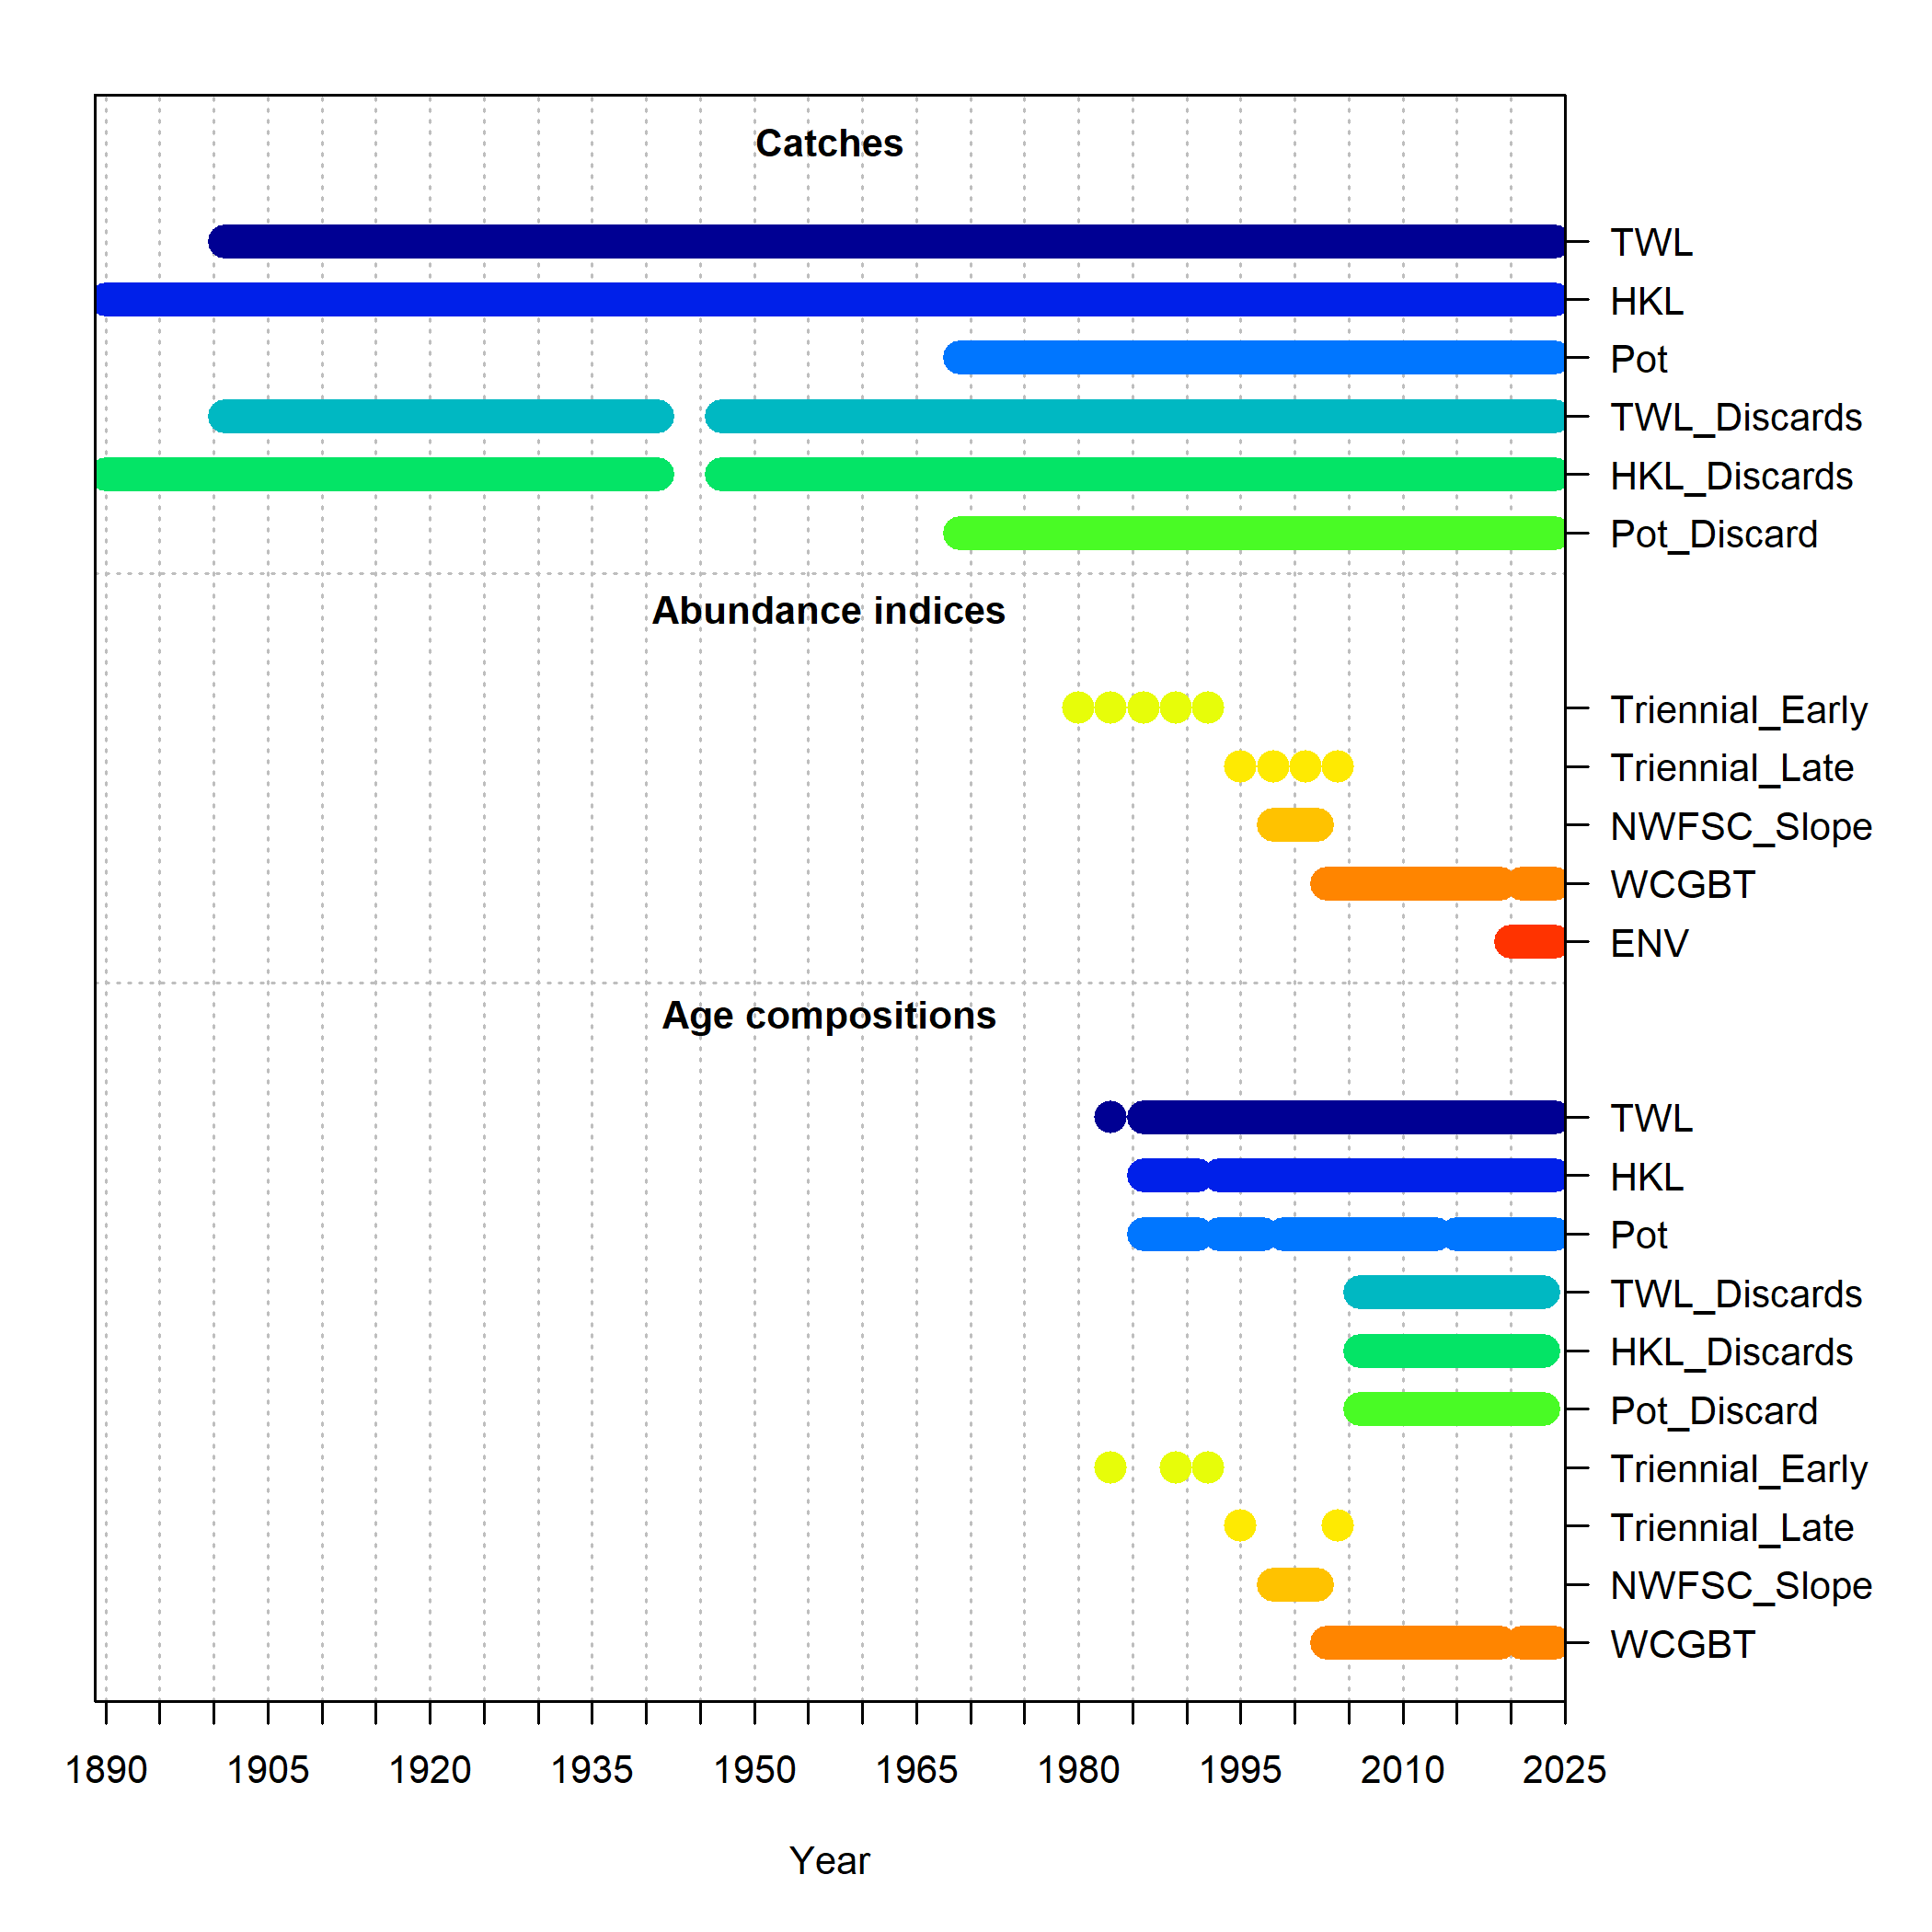
\includegraphics{../model/_bridging/13_m_prior/plots/data_plot.png}

}

\caption{\label{fig-data}Data used in the base model.}

\end{figure}%

\newpage

\begin{figure}

\centering{

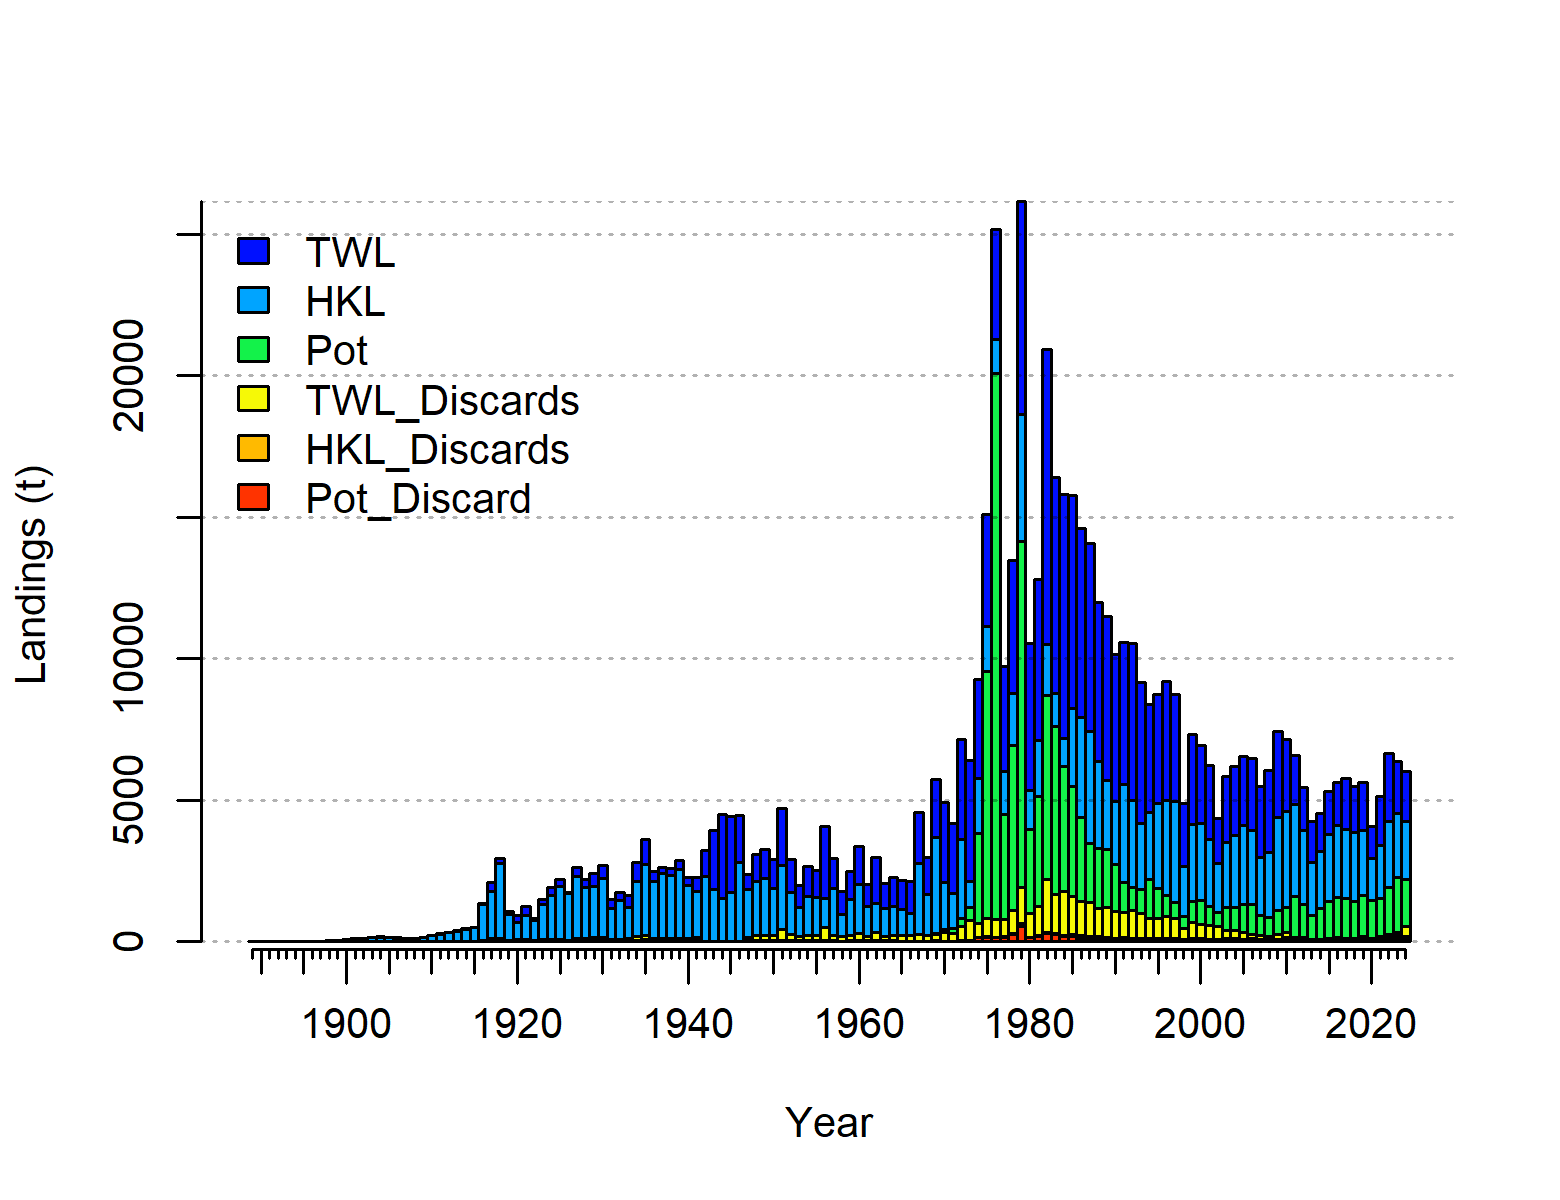
\includegraphics{../model/_bridging/13_m_prior/plots/catch2_landings_stacked.png}

}

\caption{\label{fig-landings}Landings in metric tons (mt) by year for
trawl, pot, and hook-and line gears.}

\end{figure}%

\pagebreak

\begin{figure}

\centering{


\includegraphics{../model/_bridging/13_m_prior/plots/catch16_landings_+_dead_discards.png}

}

\caption{\label{fig-catches}Catches, landed and dead discards, in metric
tons (mt) by year for trawl, pot, and hook-and line gears.}

\end{figure}%

\pagebreak

\subsection{Biology}\label{biology}

\begin{figure}

\centering{

\includegraphics{SAR_USWC_sablfefish_skeleton_files/figure-pdf/fig-maturity-data-1.pdf}

}

\caption{\label{fig-maturity-data}Samples by age that were determined to
be functionally mature and immature north and south of 36 degrees north
latitude. Immature fish have a functional maturity of 0 and mature fish
have a functional maturity of 1. Blue vertical dashed line at age 7.}

\end{figure}%

\newpage

\begin{figure}

\centering{

\includegraphics{SAR_USWC_sablfefish_skeleton_files/figure-pdf/fig-maturity-ogive-1.pdf}

}

\caption{\label{fig-maturity-ogive}Estimated maturity-at-age by area and
the biomass weighted coastwide (Spatial) maturity curve.}

\end{figure}%

\newpage

\subsection{Model Results}\label{model-results}

\subsubsection{Model Bridging}\label{model-bridging}

\subsubsection{Biology}\label{biology-1}

\subsubsection{Selectivity}\label{selectivity}

\subsubsection{Recruitment}\label{recruitment-1}

\subsubsection{Fits to Data}\label{fits-to-data}

\subsubsection{Time-series}\label{time-series}

\begin{figure}

\centering{

\includegraphics{SAR_USWC_sablfefish_skeleton_files/figure-pdf/fig-sb-1.pdf}

}

\caption{\label{fig-sb}}

\end{figure}%

\newpage

\subsubsection{Sensitivity Analyse and
Retrospectives}\label{sensitivity-analyse-and-retrospectives}

\subsubsection{Likelihood Profiles}\label{likelihood-profiles-1}

\subsubsection{Reference Points and
Forecasts}\label{reference-points-and-forecasts}

\newpage{}

\section{Notes}\label{notes}

\newpage{}

\section*{Appendices}\label{sec-appendix}
\addcontentsline{toc}{section}{Appendices}

\phantomsection\label{refs}
\begin{CSLReferences}{1}{0}
\bibitem[\citeproctext]{ref-Anderson:2022:SRP}
Anderson, Sean C., Eric J. Ward, and Philina A. English, and Lewis A. K.
Barnett. 2022. {``{sdmTMB}: An r Package for Fast, Flexible, and
User-Friendly Generalized Linear Mixed Effects Models with Spatial and
Spatiotemporal Random Fields.''} \emph{bioRxiv} 2022.03.24.485545.
\url{https://doi.org/10.1101/2022.03.24.485545}.

\bibitem[\citeproctext]{ref-bradburn_2003_2011}
Bradburn, M. J., A. A Keller, and B. H. Horness. 2011. {``The 2003 to
2008 {US} {West} {Coast} Bottom Trawl Surveys of Groundfish Resources
Off {Washington}, {Oregon}, and {California}: Estimates of Distribution,
Abundance, Length, and Age Composition.''} US Department of Commerce,
National Oceanic; Atmospheric Administration, National Marine Fisheries
Service.

\bibitem[\citeproctext]{ref-browning_fisheries_1980}
Browning, R. J. 1980. {``Fisheries of the {N}orth {P}acific: History,
Species, Gear, \& Processes.''} Anchorage, AK: Alaska Northwest
Publishing Company.

\bibitem[\citeproctext]{ref-echave_interdecadal_2012}
Echave, K. B., D. H. Hanselman, M. D. Adkison, and M. F. Sigler. 2012.
{``Interdecadal Change in Growth of Sablefish (\emph{{A}noplopoma
Fimbria}) in the Northeast {P}acific {O}cean.''} \emph{Fisheries
Bulletin} 210: 361--74.

\bibitem[\citeproctext]{ref-eschmeyer_field_1983}
Eschmeyer, W. N\textgreater, and E. S. Herald. 1983. \emph{A Field Guide
of {Pacific} Coast Fishes {North} {America}}. Boston, MA: Houghton
Mifflin CO.

\bibitem[\citeproctext]{ref-fujioka_description_1988}
Fujioka, J. T., F. R. Shaw, G. A. McFarlane, T. Sasaki, and B. E.
Bracken. 1988. {``Description and Summary of the {C}anadian, {J}apanese
and {U}.{S}. Joint Data Base of Sablefish Tag Releases and Recoveries
During 1977-1983.''} NMFS F/NWC-137. {U}.{S}. Department of Commerce.

\bibitem[\citeproctext]{ref-gertseva_spatial_2017}
Gertseva, V. V., S. E. Matson, and J. Cope. 2017. {``Spatial Growth
Variability in Marine Fish: Example from {N}ortheast {P}acific
Groundfish.''} \emph{{ICES} Journal of Marine Science} 74 (6): 1602--13.

\bibitem[\citeproctext]{ref-guzman_reproductive_2017}
Guzmán, J. M., J. A. Luckenback, M. A. Middleton, K. C. Massee, C.
Jensen, F. W. Goetz, A. J. Jasonowicz, and P. Swanson. 2017.
{``Reproductive Life History of Sablefish (\emph{{A}noplopoma Fimbria})
from the {U}.{S}. {W}ashington Coast.''} \emph{{PLOS} One} 12 (9):
0184413. \url{https://doi.org/10.1371/journal.pone.0184413}.

\bibitem[\citeproctext]{ref-hamel_development_2022}
Hamel, Owen S., and Jason M. Cope. 2022. {``Development and
Considerations for Application of a Longevity-Based Prior for the
Natural Mortality Rate.''} \emph{Fisheries Research} 256 (December):
106477. \url{https://doi.org/10.1016/j.fishres.2022.106477}.

\bibitem[\citeproctext]{ref-hanselman_move_2015}
Hanselman, D. H., J. Heifetz, K. B. Echave, and S. C. Dressel. 2015.
{``Move It or Lose It: Movement and Mortality of Sablefish Tagged in
{A}laska.''} \emph{Canadian Journal of Fish and Aquatic Sciences} 72:
238--51. \url{https://doi.org/10.1139/cjfas-2014-0251}.

\bibitem[\citeproctext]{ref-hart_pacific_1973}
Hart, J. L. 1973. {``Pacific Fishes of {C}anada.''} 180. St. Andrews,
NB, Canada: Fisheries Research Board of Canada Bulletin.

\bibitem[\citeproctext]{ref-head_maturity_2014}
Head, M. A., A. A. Keller, and M. Bradburn. 2014. {``Maturity and Growth
of Sablefish, \emph{{A}noplopoma Fimbria}, Along the {U.S.} {W}est
{C}oast.''} \emph{Fisheries Research} 159: 56--67.

\bibitem[\citeproctext]{ref-heifetz_movement_1991}
Heifetz, J., and J. T. Fujioka. 1991. {``Movement Dynamics of Tagged
Sablefish in the Northeastern {P}acific.''} \emph{Fisheries Research}
11: 355--74.

\bibitem[\citeproctext]{ref-jasonowicz_love_2017}
Jasonowicz, A. J., F. W. Goetz, G. W. Goetz, and K. M. Nichols. 2017.
{``Love the One You're with: Genomic Evidence of Panmixia in the
Sablefish (\emph{{A}noplopoma Fimbria}).''} \emph{Canadian Journal of
Fisheries and Aquatic Science} 74: 377--87.

\bibitem[\citeproctext]{ref-kapur_oceanographic_2020}
Kapur, M, M Haltuch, B Connors, L Rogers, A Berger, E Koontz, J Cope, et
al. 2020. {``{Oceanographic features delineate growth zonation in
Northeast Pacific sablefish}.''} \emph{Fisheries Research} 222 (July).
\url{https://doi.org/10.1016/j.fishres.2019.105414}.

\bibitem[\citeproctext]{ref-karnowski_historical_2014}
Karnowski, M., V. V. Gertseva, and Andi Stephens. 2014. {``Historical
{Reconstruction} of {Oregon}'s {Commercial} {Fisheries} {Landings}.''}
Salem, OR: Oregon Department of Fish; Wildlife.

\bibitem[\citeproctext]{ref-low_sablefish_1976}
Low, L. L., G. K. Tanonaka, and H. H. Shippen. 1976. {``Sablefish of the
{N}ortheastern {P}acific {O}cean and {B}ering {S}ea.''} Seattle, WA:
{U}.{S}. Department of Commerce.

\bibitem[\citeproctext]{ref-lynde_historical_1986}
Lynde, M. V. H. 1986. {``The Historical Annotated Landings ({HAL})
Database: Documentation of Annual Harvest of Groundfish from the
Northeast {P}acific and Eastern {B}ering {S}ea from 1956 to 1980.''}
NMFS F/NWC-103. Seattle, WA: {U}.{S}. Department of Commerce.

\bibitem[\citeproctext]{ref-mcdevitt_status_1987}
McDevitt, S. A. 1987. {``The Status of the Sablefish Resource in Waters
Off the {U}.{S}. {W}est {C}oast.''} Portland, OR: Pacific Fishery
Management Council.
\url{http://www.pcouncil.org/groundfish/stock-assessments/}.

\bibitem[\citeproctext]{ref-methot_assessment_1994}
Methot, R. D. 1994. {``Assessment of the West Coast Sablefish Stock in
1994.''} Portland, OR: Pacific Fishery Management Council.
\url{http://www.pcouncil.org/groundfish/stock-assessments/}.

\bibitem[\citeproctext]{ref-morita_sex_2012}
Morita, S. H., K. Morita, and A. Nishimura. 2012. {``Sex-Biased
Dispersal and Growth in Sablefish (\emph{{A}noplopoma Fimbria}) in the
Northeastern {P}acific {O}cean.''} \emph{Environmental Biology of
Fishes} 94: 505--11.

\bibitem[\citeproctext]{ref-pikitch_evaluation_1988}
Pikitch, Ellen K., Daniel L. Erickson, and John R. Wallace. 1988. {``An
Evaluation of the Effectiveness of Trip Limits as a Management Tool.''}
88-27. Northwest; Alaska Fisheries Center, National Marine Fisheries
Service NWAFC Processed Report.
\url{https://www.afsc.noaa.gov/Publications/ProcRpt/PR1988-27.pdf}.

\bibitem[\citeproctext]{ref-punt_quantifying_2008}
Punt, A. E., D. C. Smith, K. KrusicGolub, and S. Robertson. 2008.
{``Quantifying Age-Reading Error for Use in Fisheries Stock Assessments,
with Application to Species in {A}ustralia's Southern and Eastern
Scalefish and Shark Fishery.''} \emph{Canadian Journal of Fisheries and
Aquatic Sciences} 65 (9): 1991--2005.
\url{https://doi.org/10.1139/F08-111}.

\bibitem[\citeproctext]{ref-ralston_documentation_2010}
Ralston, Stephen, Don E. Pearson, John C. Field, and Meisha Key. 2010.
{``Documentation of the {California} Catch Reconstruction Project.''} US
Department of Commerce, National Oceanic; Atmospheric Adminstration,
National Marine.

\bibitem[\citeproctext]{ref-rogers_numerical_1992}
Rogers, Jean Beyer, and Ellen K. Pikitch. 1992. {``Numerical Definition
of Groundfish Assemblages Caught Off the Coasts of {Oregon} and
{Washington} Using Commercial Fishing Strategies.''} \emph{Canadian
Journal of Fisheries and Aquatic Sciences} 49 (12): 2648--56.

\bibitem[\citeproctext]{ref-shaw_movement_1997}
Shaw, F. R., and N. B. Parks. 1997. {``Movement Patterns of Tagged
Sablefish, \emph{{A}noplopoma Fimbria}, Recovered on Seamounts in the
{N}ortheast {P}acific {O}cean and {G}ulf of {A}laska.''} NMFS 130.
Seattle, WA: {U}.{S}. Department of Commerce.

\bibitem[\citeproctext]{ref-sogard_patterns_2017}
Sogard, S. M., and S. A. Berkeley. 2017. {``Patterns of Movement,
Growth, and Survival of Adult Sablefish (\emph{{A}noplopoma Fimbria}) at
Contrasting Depths in Slope Waters Off {O}regon.''} \emph{Fisheries
Bulletin} 115: 233--51.

\bibitem[\citeproctext]{ref-then_evaluating_2015}
Then, A. Y., J. M. Hoenig, N. G. Hall, and D. A. Hewitt. 2015.
{``Evaluating the Predictive Performance of Empirical Estimators of
Natural Mortality Rate Using Information on over 200 Fish Species.''}
\emph{ICES Journal of Marine Science} 72 (1): 82--92.
\url{https://doi.org/10.1093/icesjms/fsu136}.

\bibitem[\citeproctext]{ref-tolimieri_oceanographic_2018}
Tolimieri, N., M. A. Haltuch, Q. Lee, M. G. Jacox, and S. J. Bograd.
2018. {``\href{}{Oceanographic Drivers of Sablefish Recruitment in the
{C}alifornia {C}urrent}.''} \emph{Fisheries Oceanography} 27: 458--74.

\bibitem[\citeproctext]{ref-weinberg_estimation_2002}
Weinberg, James R., Paul J. Rago, W. Waldo Wakefield, and Charles Keith.
2002. {``Estimation of Tow Distance and Spatial Heterogeneity Using Data
from Inclinometer Sensors: An Example Using a Clam Survey Dredge.''}
\emph{Fisheries Research} 55 (1--3): 49--61.
\url{https://doi.org/10.1016/S0165-7836(01)00292-2}.

\end{CSLReferences}




\end{document}
